\documentclass[xcolor=dvipsnames]{beamer}
\mode<presentation>
{ 
 \usetheme{Dresden}
 \usecolortheme[named=OliveGreen]{structure}
}
\usepackage{pgf,pgfarrows,pgfnodes,pgfautomata,pgfheaps,pgfshade}
\usepackage{amsmath,amsthm,amssymb,amsfonts}
\usepackage[czech]{babel}
%\usepackage[cp1250]{inputenc} 	% kodovani cestiny MS Windows
%\usepackage[latin2]{inputenc} 	% kodovani cestiny Linux
\usepackage[utf8]{inputenc}
\usepackage{times}
\usepackage[T1]{fontenc}
\usepackage{xspace}
\usepackage{color}
\usepackage{epstopdf}
\usepackage{ulem} %kvuli preskrtnutemu textu
\usepackage{comment}
\usepackage{lmodern}
\usepackage{graphicx}
\usepackage{xcolor}


\newtheorem{veta}{Věta} 
\newtheorem{lema}[veta]{Lemma}
\newtheorem{dusledek}[veta]{Důsledek}
\theoremstyle{definition} \newtheorem{definice}[veta]{Definice}
\newtheorem{priklad}{Příklad}
\theoremstyle{remark}
\newtheorem*{poznamka}{Poznámka}
\newtheorem*{reseni}{Řešení}  

\title[Rovnovážné modely v teorii portfolia]
{Rovnovážné modely v teorii portfolia}
\author[Lenka Křivánková]
{Lenka Křivánková}
\institute[SCI MUNI]
{ \begin{figure}[!htbp] 
 \centering
 
\includegraphics[width=2cm]{IMG/znak_MU_cerny.pdf} \qquad\qquad
 \includegraphics[width=3cm]{IMG/personal_finance-3.jpg}\qquad\qquad
 
\includegraphics[width=2cm]{IMG/znak_PrF_cerny.pdf}  
\end{figure} 
}
\date[3. 9. 2013]
{\scriptsize{31. května 2016, Bratislava}}

%\AtBeginSubsection[]
%{
%  \begin{frame}<beamer>
%    \frametitle{Content}
%    \tableofcontents[currentsection,currentsubsection]
%  \end{frame}
%}

\AtBeginSection[]
{
\begin{frame}<beamer>
  \frametitle{Obsah}
  \tableofcontents[currentsection]
\end{frame}
}

\renewcommand{\vec}[1]{\mathchoice{\mbox{\boldmath$\displaystyle#1$}}
{\mbox{\boldmath$\textstyle#1$}}
{\mbox{\boldmath$\scriptstyle#1$}}
{\mbox{\boldmath$\scriptscriptstyle#1$}}}


\begin{document}

%\begin{itemize}[<+->]
  % \item
  %\end{itemize}

\begin{frame}
  \titlepage
\end{frame}

\begin{frame}
  \frametitle{Obsah}
  \tableofcontents
  % You might wish to add the option [pausesections] 
\end{frame}

\section{Portfolio a jeho charakteristiky}

\subsection{Definice portfolia}

\begin{frame}
  \frametitle{Portfolio}
  %\textcolor{RedOliveGreen}{Portfolio} is 
  \begin{itemize}
   \item množina aktiv (akcií, dluhopisů, peněz...)
  \end{itemize}

 \begin{figure}[!htbp]
  \centering 
  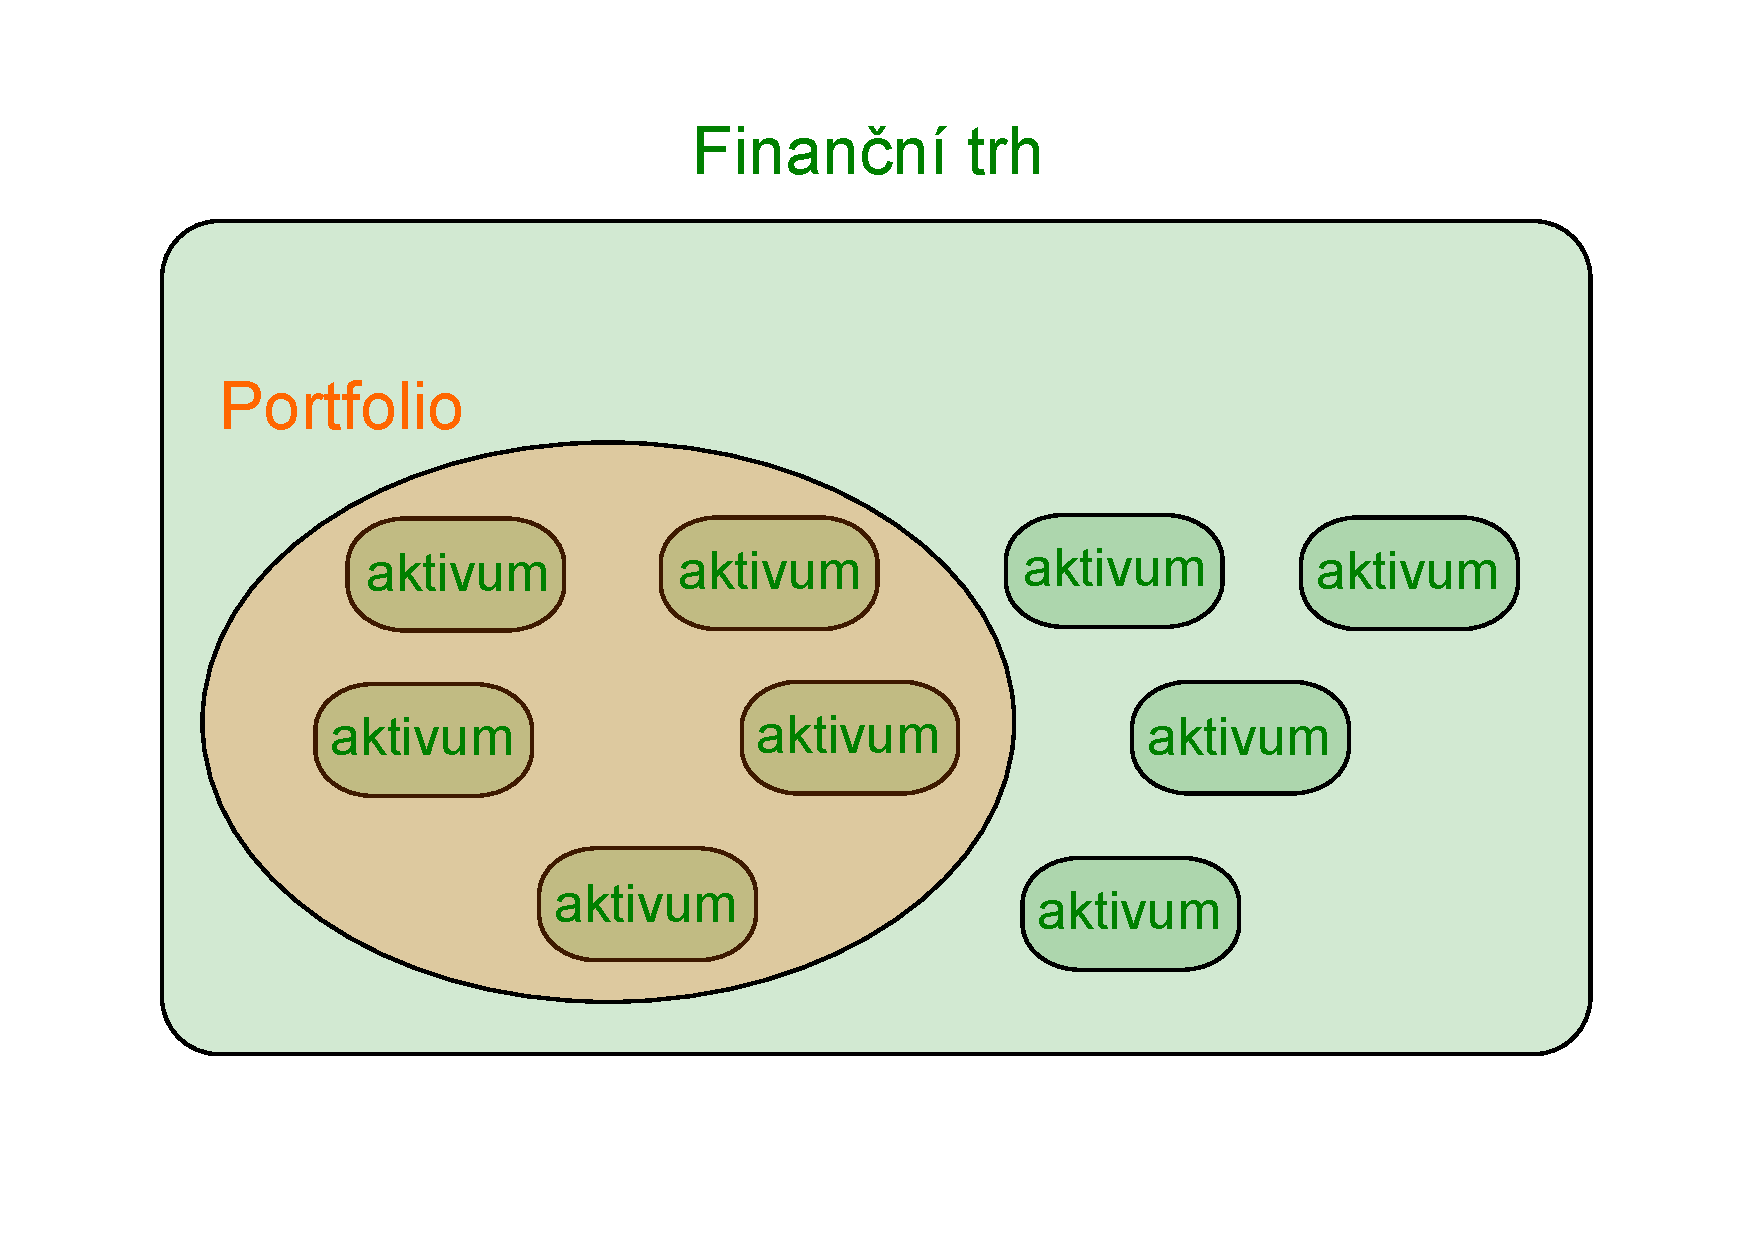
\includegraphics[width=9cm]{IMG/portfolio.pdf}
  %\caption{}
 \end{figure}
\end{frame}


\begin{frame}
  \frametitle{Portfolio}
  %\textcolor{RedOliveGreen}{Portfolio} is 
  %\begin{itemize}
   %\item množina aktiv (akcií, dluhopisů, peněz...)
  %\end{itemize}

 \begin{figure}[!htbp]
  \centering 
  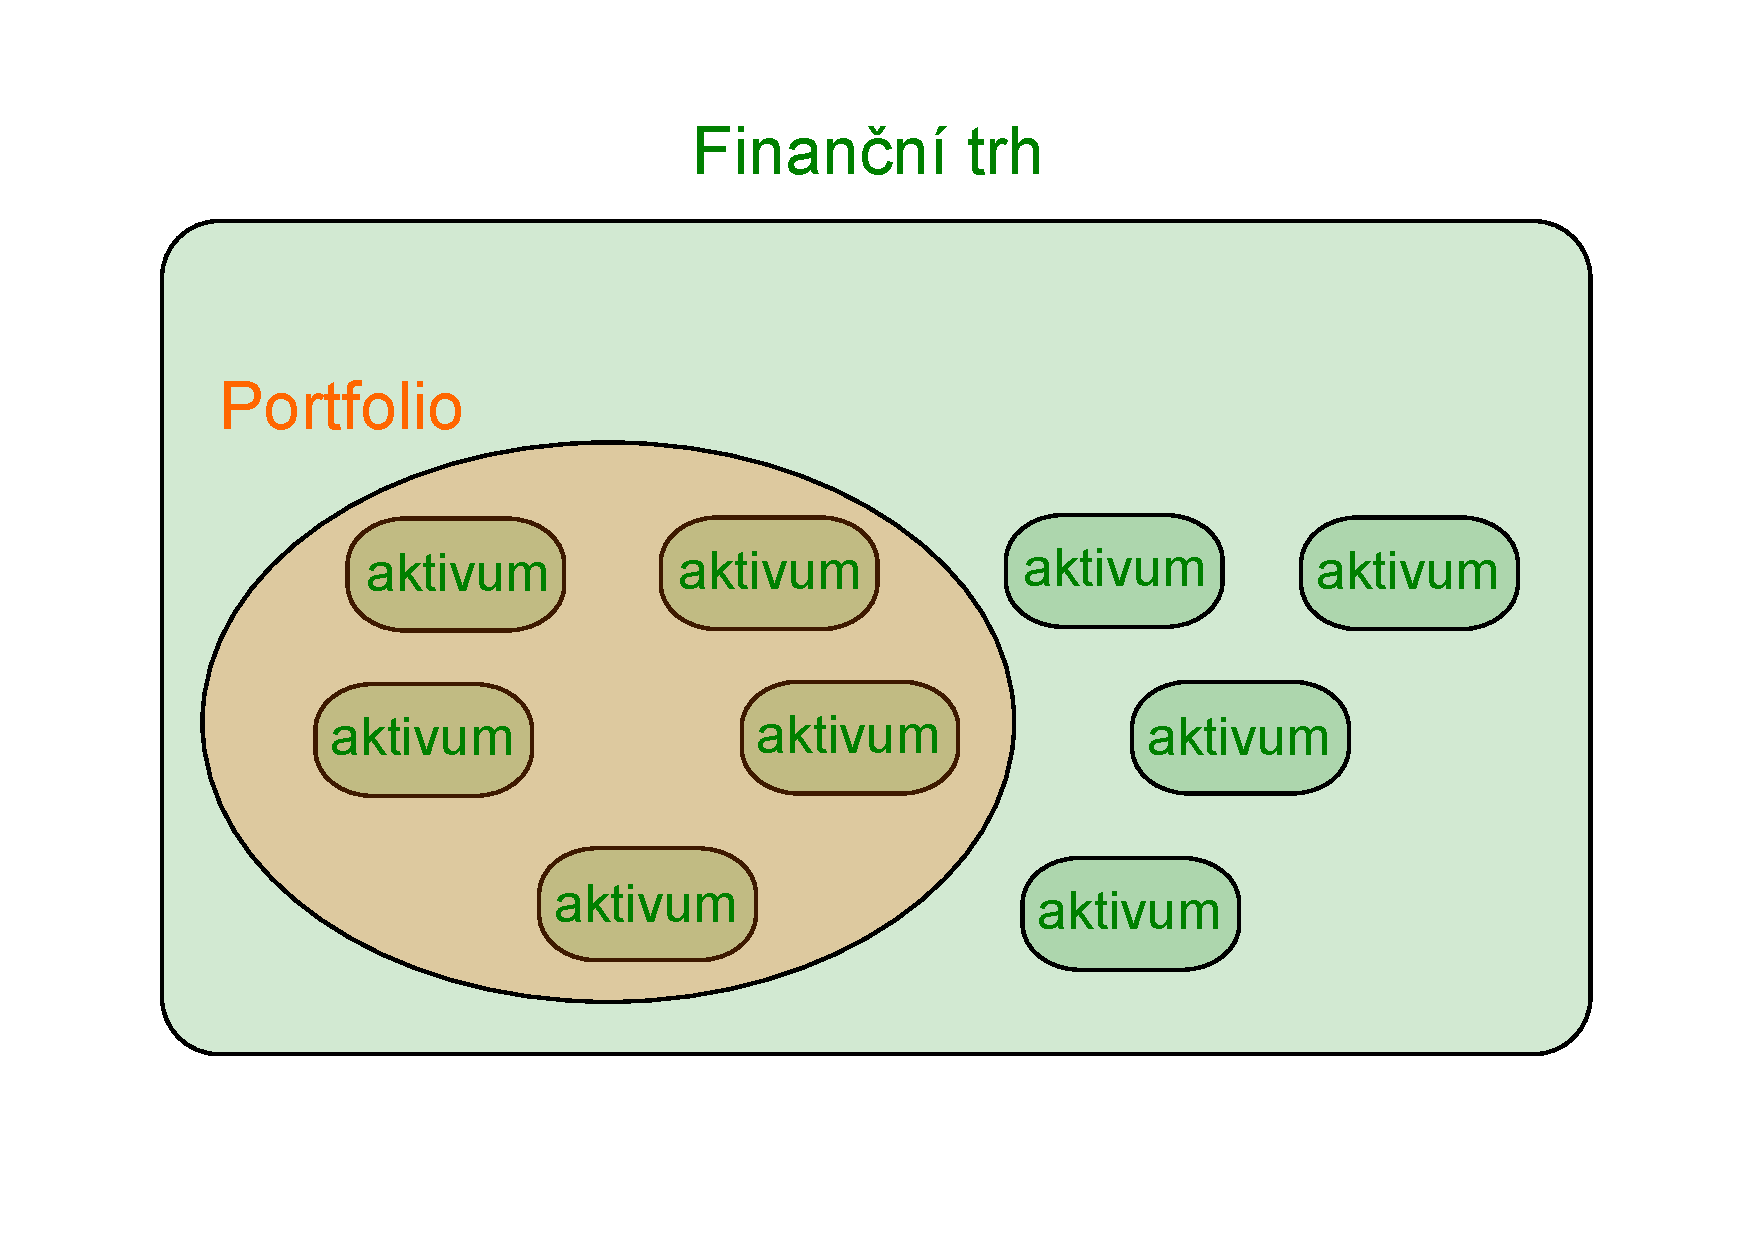
\includegraphics[width=7cm, clip, trim= 0 80 0 60]{IMG/portfolio.pdf}
  %\caption{}
 \end{figure}

\textcolor{OliveGreen}{Váhy portfolia}
   \begin{itemize}
    \item relativní podíly aktiv obsažených v portfoliu
    \item $\boldsymbol{X}=(X_1,\dots,X_n)^\mathrm{T}$, kde $\sum_{j=1}^nX_j=1$
   \end{itemize}
\end{frame}


\begin{frame}
  \frametitle{Výnosnost a riziko}
  \begin{figure}[!htbp]
  \centering 
  
\includegraphics[width=6cm]{IMG/houpacka.jpg}
  %\caption{}
 \end{figure}
\end{frame}

\subsection{Výnosnost a riziko aktiv}

\begin{frame}
  \frametitle{Výnosnost aktiva}
  \textcolor{OliveGreen}{Míra výnosnosti}
    \begin{itemize}
   \item relativní zisk nebo ztráta z investice
   \item náhodná veličina $r_j$
   \item očekávaná výnosnost $\mathsf{E}(r_j)=\mu_j$
   \item rozptyl výnosnosti $\mathsf{D}(r_j)=\sigma_j^2$
   \item $r_j(t,t+\Delta t)=\frac{P_j(t+\Delta t)-P_j(t)}{P_j(t)}$      
  \end{itemize}
\end{frame}
  
\begin{frame}
  \frametitle{Riziko aktiva}
  \textcolor{OliveGreen}{Riziko}
  \begin{itemize}
   \item směrodatná odchylka výnosnosti aktiva 
   \item $\sqrt{\mathsf{D}(r_j)}=\sigma_j$   
  \end{itemize}
\end{frame}

\subsection{Výnosnost a riziko portfolia}

\begin{frame}
 \frametitle{Výnosnost portfolia}
% \textcolor{OliveGreen}{Váhy portfolia}
%   \begin{itemize}
%    \item relativní podíly aktiv obsažených v portfoliu
%    \item $\boldsymbol{X}=(X_1,\dots,X_n)^\mathrm{T}$, kde $\sum_{j=1}^nX_j=1$
%   \end{itemize}

   \textcolor{OliveGreen}{Výnosnost portfolia}
   \begin{itemize}
    \item náhodná veličina $r_p=\sum_{j=1}^nX_jr_j$
    \item očekávaná výnosnost portfolia $\mathsf{E}(r_p)=\mu_p=\sum_{j=1}^nX_j\mu_j$
    \item rozptyl výnosnosti portfolia $\mathsf{D}(r_p)=\sigma_p^2$ 
  \end{itemize}
\end{frame}

\begin{frame}
 \frametitle{Riziko portfolia}
  \textcolor{OliveGreen}{Riziko}
  \begin{itemize}
   \item směrodatná odchylka výnosnosti portfolia $\sqrt{\mathsf{D}(r_p)}=\sigma_p$
   \item $\sigma_p=\sqrt{\sum_{j=1}^n\sum_{k=1}^nX_jX_k\sigma_{jk}},$ \\
         kde $\mathsf{C}(r_j,r_k)=\sigma_{jk}$  je kovariance výnosností aktiva $j$ a~aktiva~$k$    
  \end{itemize}
\end{frame}

\section{Klasická teorie portfolia}

\begin{frame}
  \frametitle{Moderní teorie portfolia}
   \begin{itemize}
   \item Harry Markowitz (1952)
   \item Tobinův model (1958)
   \item CAPM - Sharpe (1964), Lintner (1965) a Mossin (1966)
  \end{itemize}
\end{frame}

\subsection{Markowitzův model}

\begin{frame}
  \frametitle{Markowitzova teorie portfolia}
  \begin{itemize}
   \item prostor výnosnost-riziko 
  \end{itemize}

 \begin{figure}[!htbp]
  \centering 
  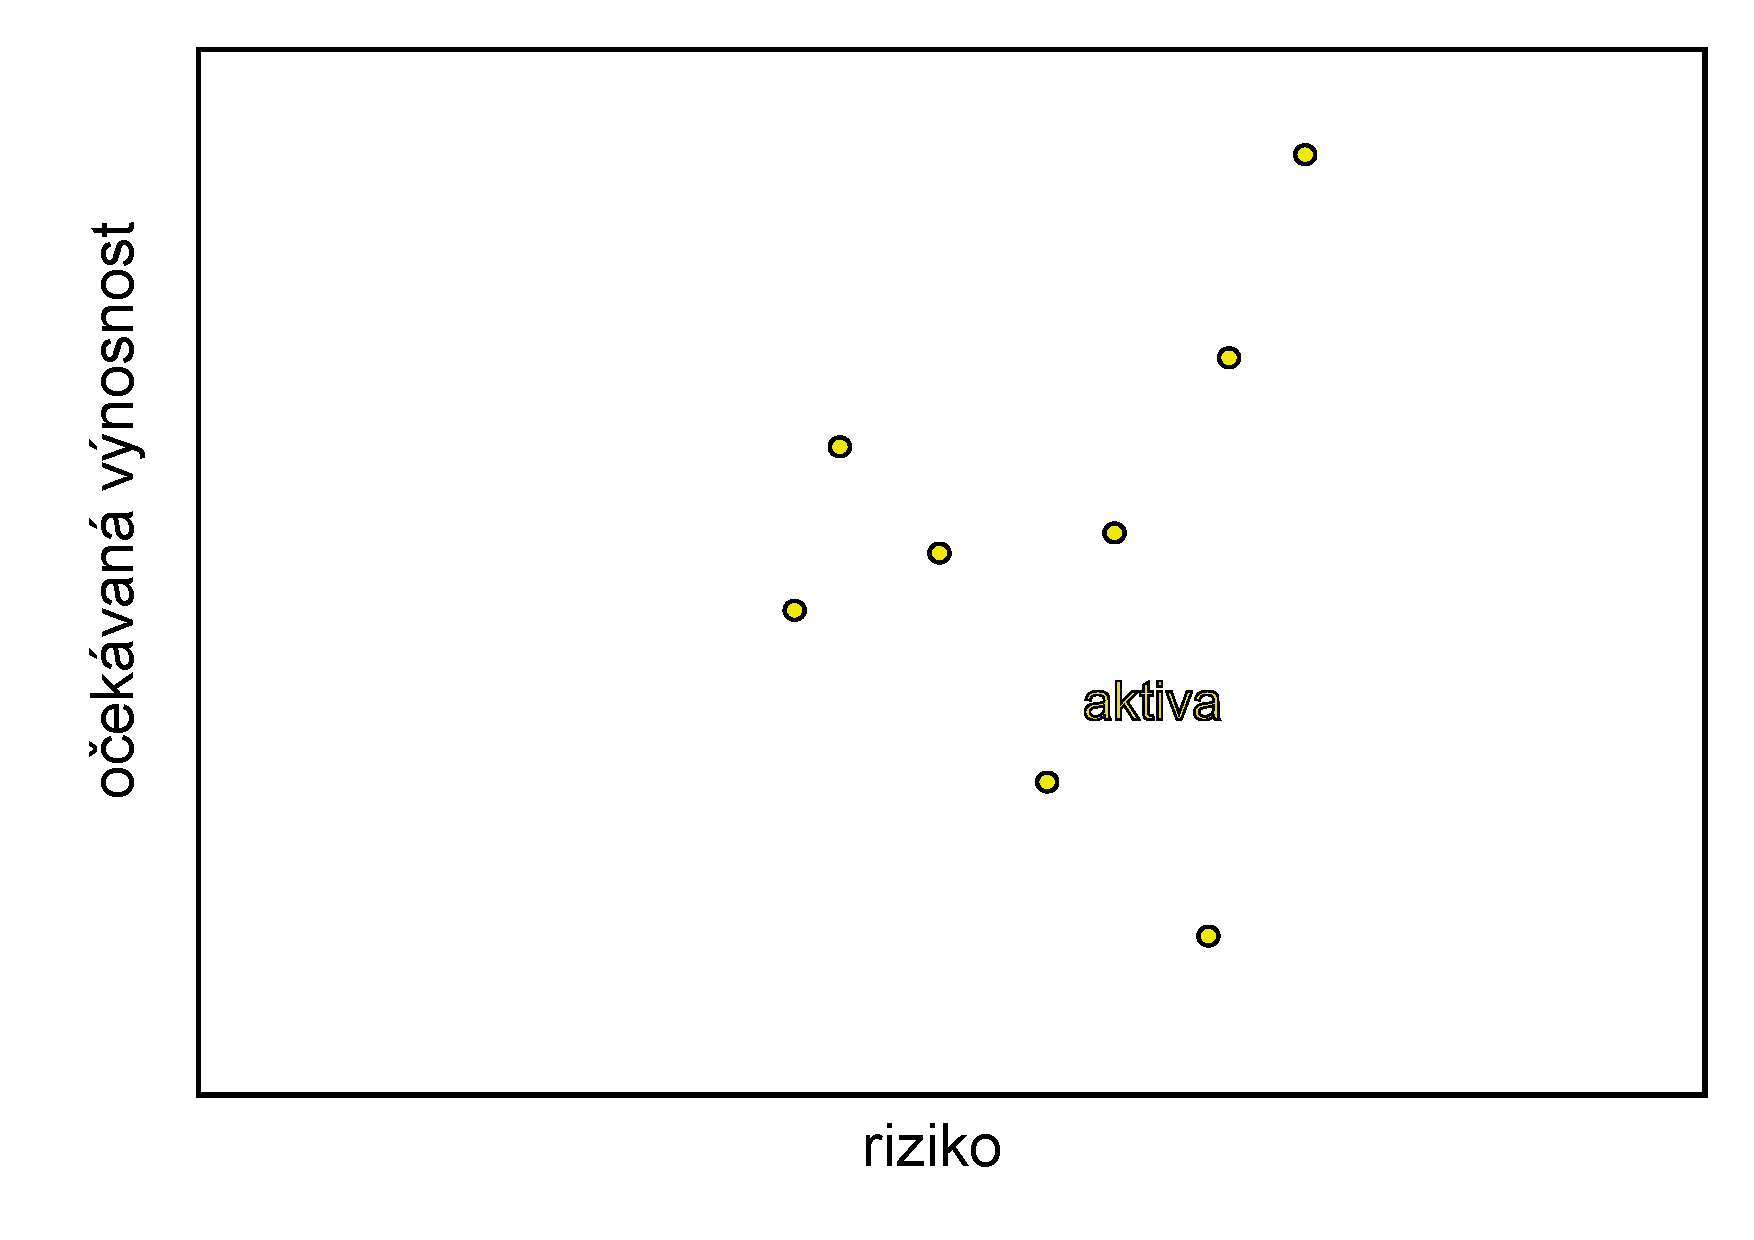
\includegraphics[width=7cm]{IMG/graf_4a.pdf}
  %\caption{}
 \end{figure}
\end{frame}

\begin{frame}                     
  \frametitle{Markowitzova teorie portfolia}
  \begin{itemize}
   \item množina přípustných portfolií 
  \end{itemize}

  \begin{figure}[!htbp]
  \centering 
  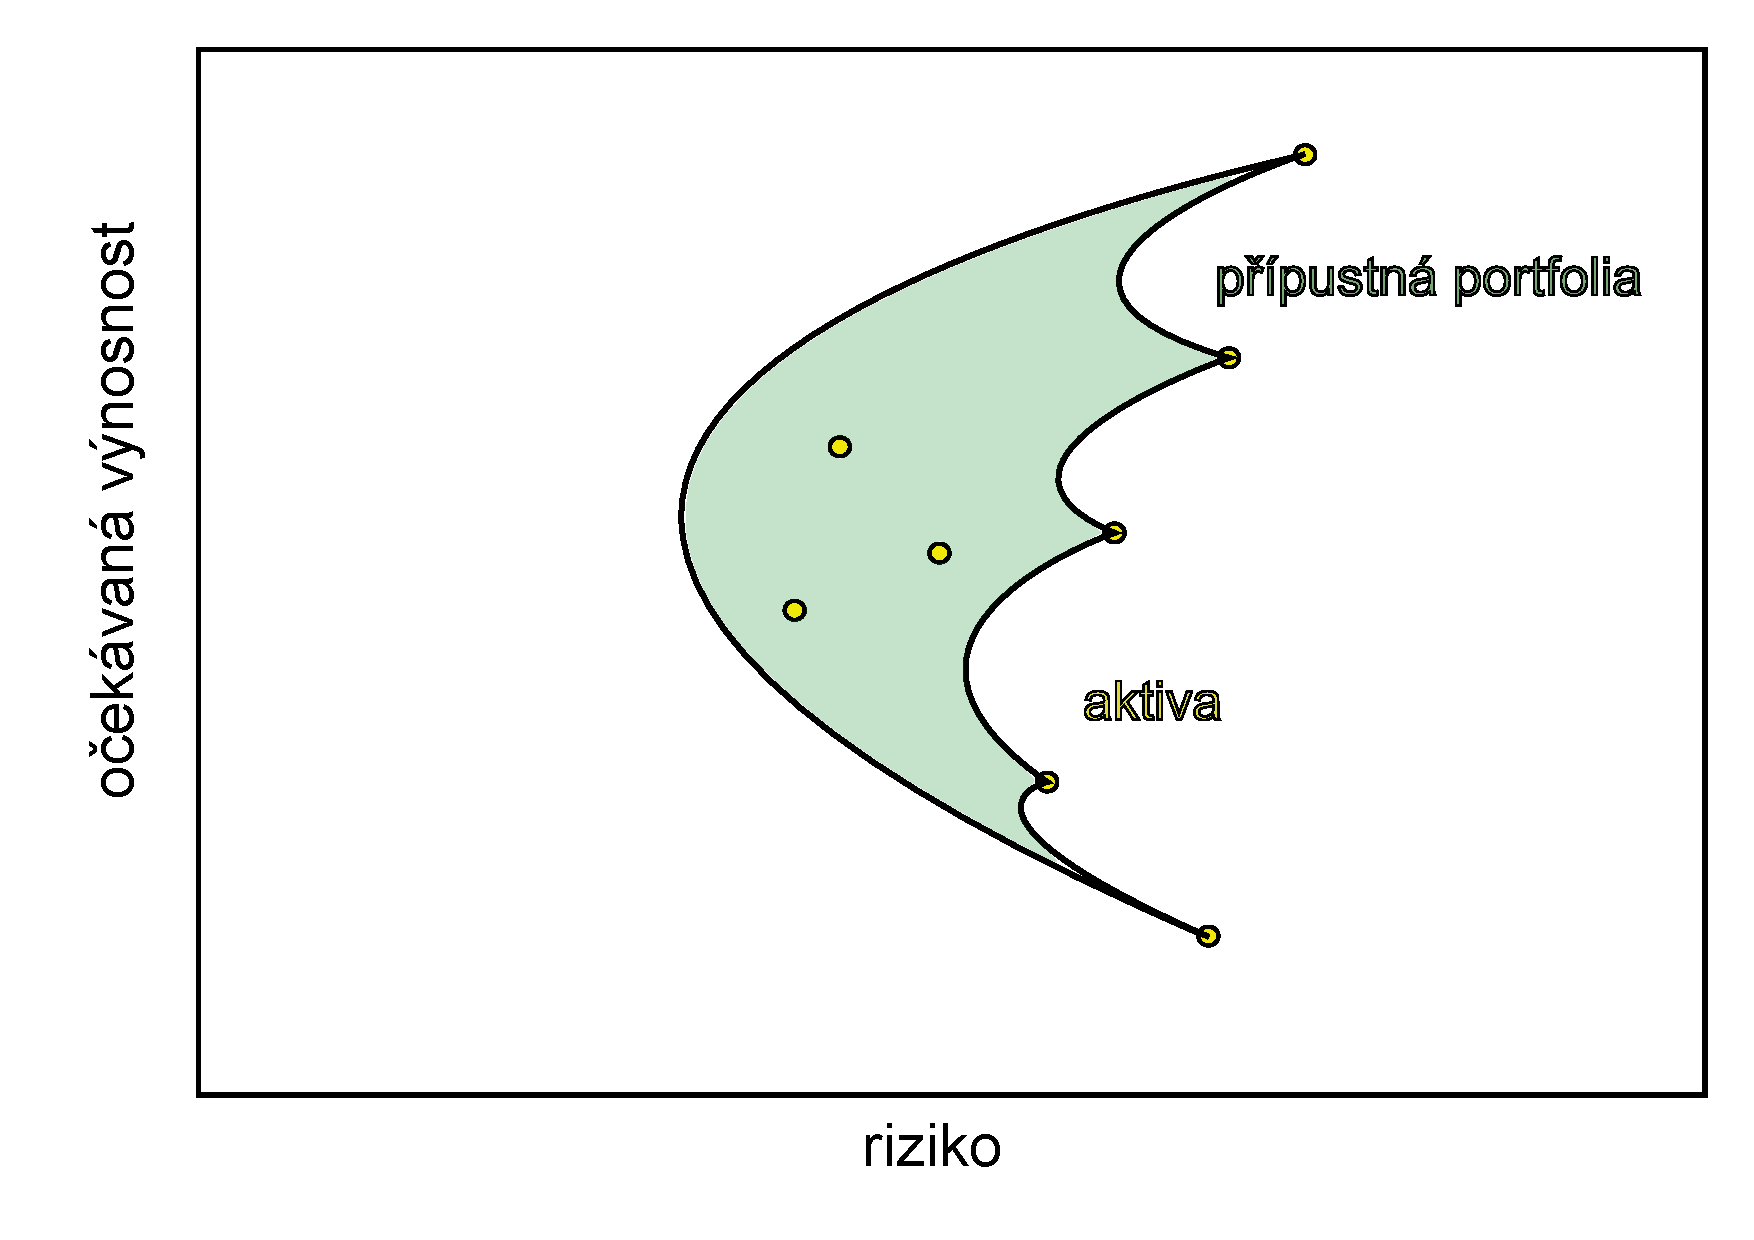
\includegraphics[width=7cm]{IMG/graf_3a.pdf}
  %\caption{}
 \end{figure}
\end{frame}

\begin{frame}
  \frametitle{Markowitzova teorie portfolia}
  \begin{itemize}
   \item množina efektivních portfolií 
  \end{itemize}
  
  \begin{figure}[!htbp]
  \centering 
  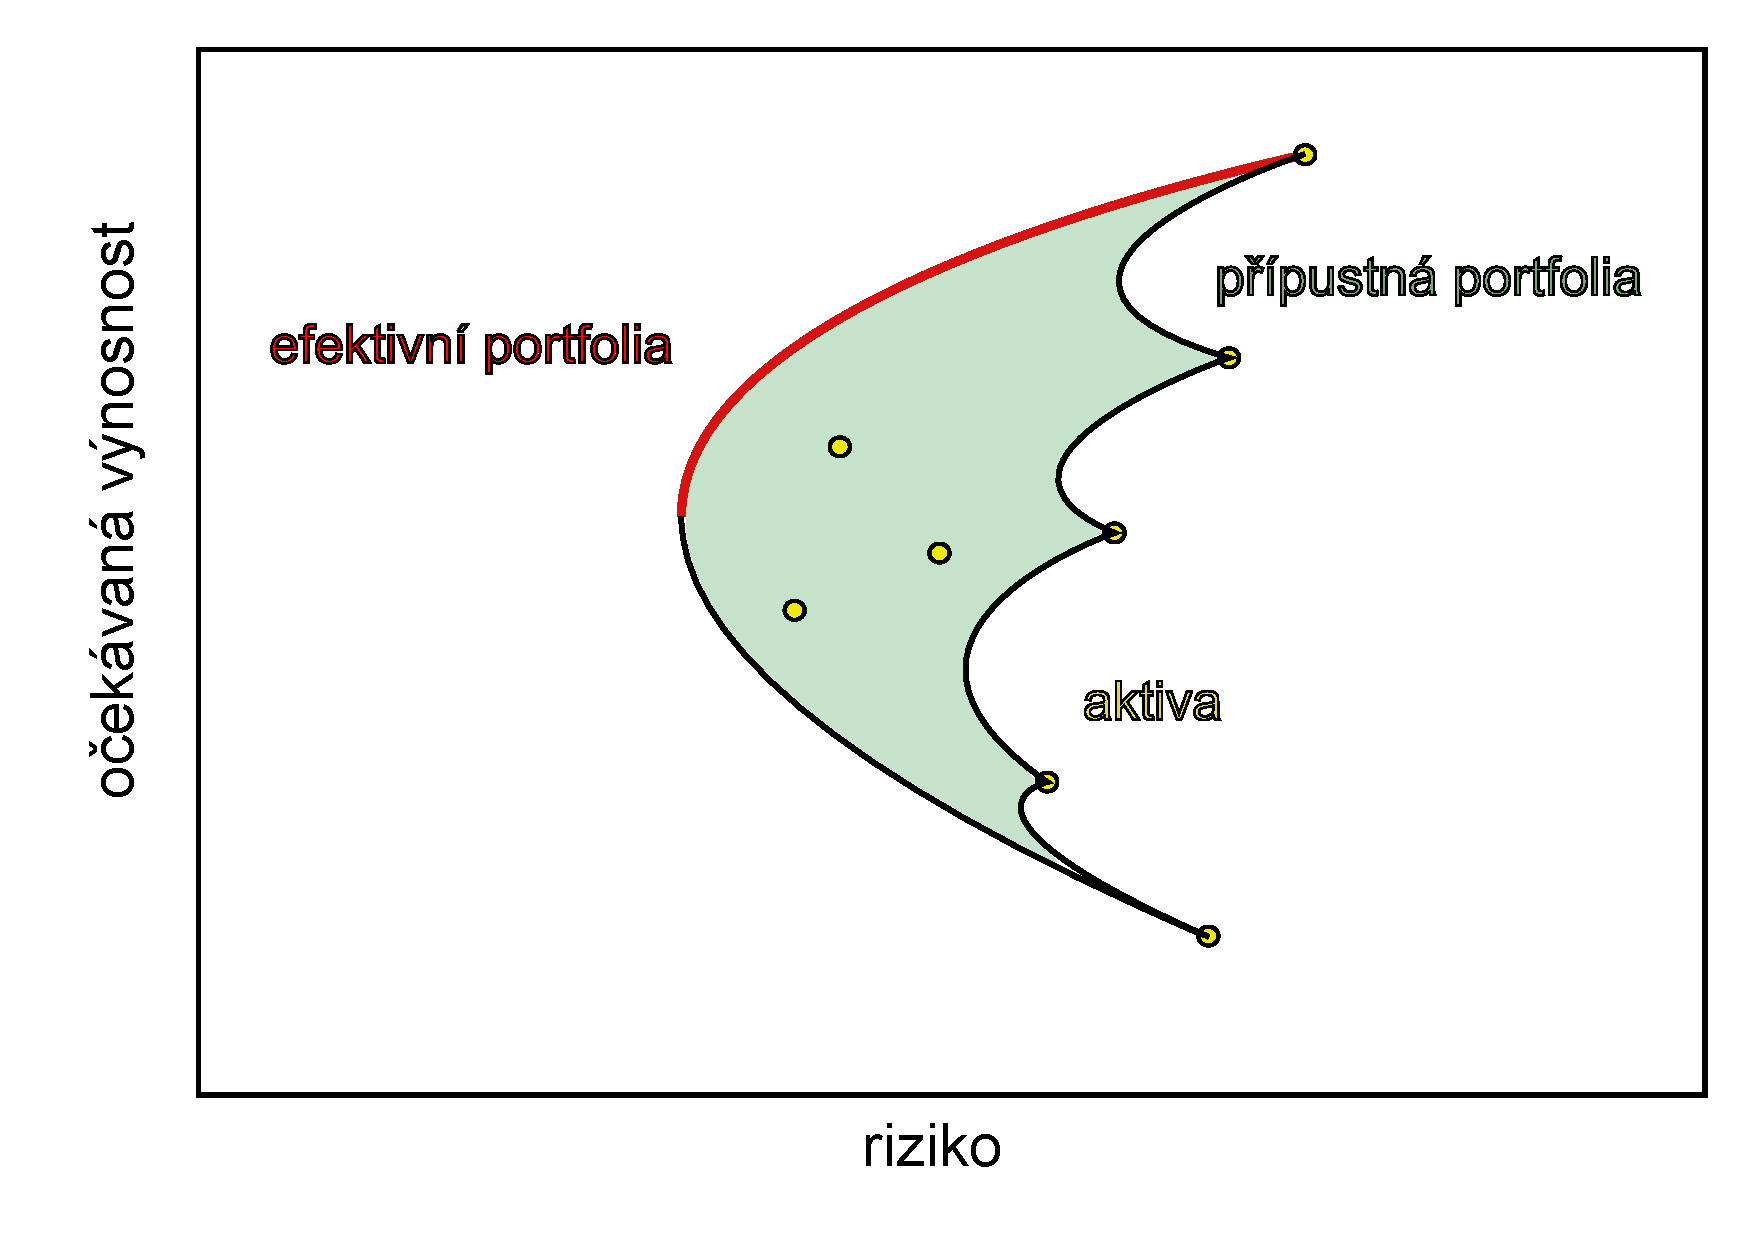
\includegraphics[width=7cm]{IMG/graf_2a.pdf}
  %\caption{}
 \end{figure}
\end{frame}

\subsection{Tobinův model}

\begin{frame}
  \frametitle{Tobinův model}
  \begin{itemize}
   \item rizikově neutrální aktivum 
  \end{itemize}
  
  \begin{figure}[!htbp]
  \centering 
  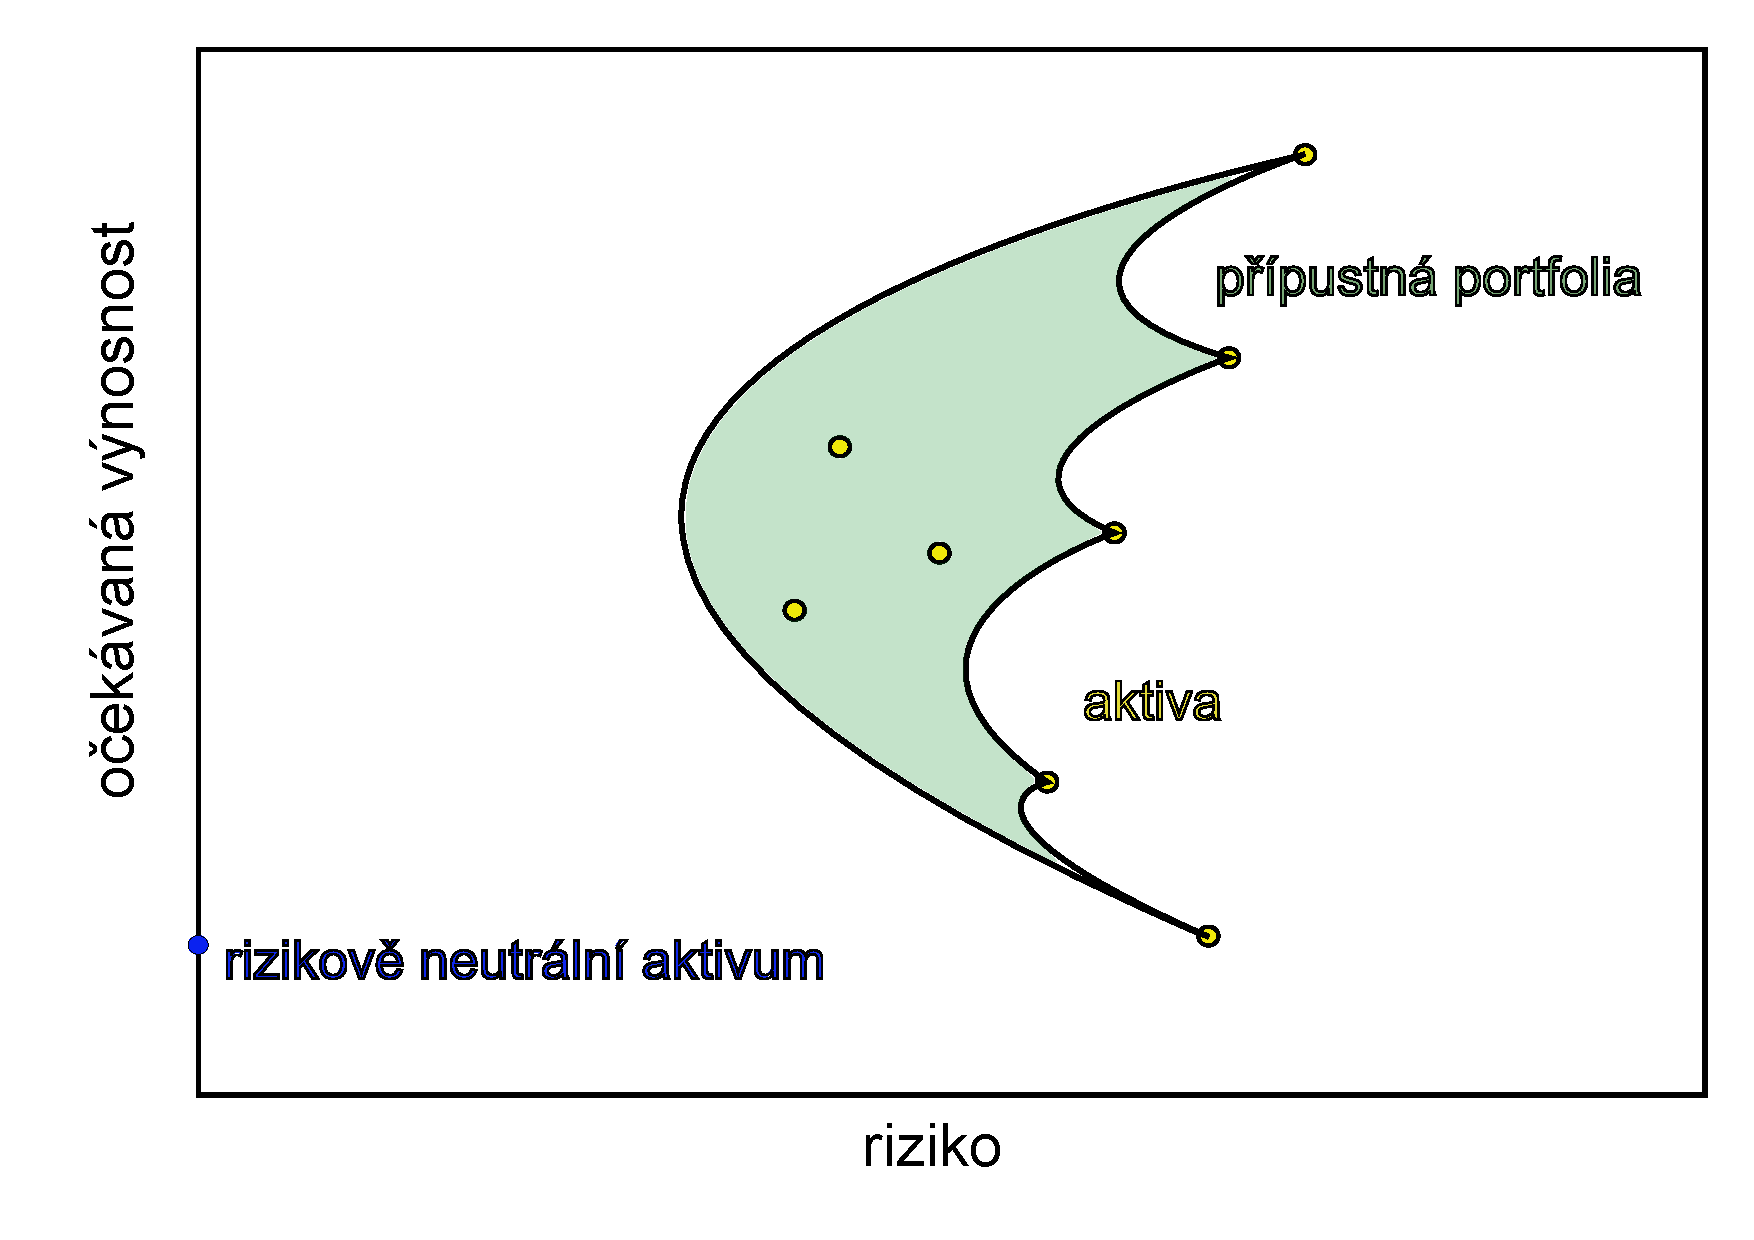
\includegraphics[width=7cm]{IMG/graf_6a.pdf}
  %\caption{}
 \end{figure}
\end{frame}

\begin{frame}
  \frametitle{Tobinův model}
  \begin{itemize}
   \item množina efektivních portfolií
  \end{itemize}  
  
  \begin{figure}[!htbp]
  \centering 
  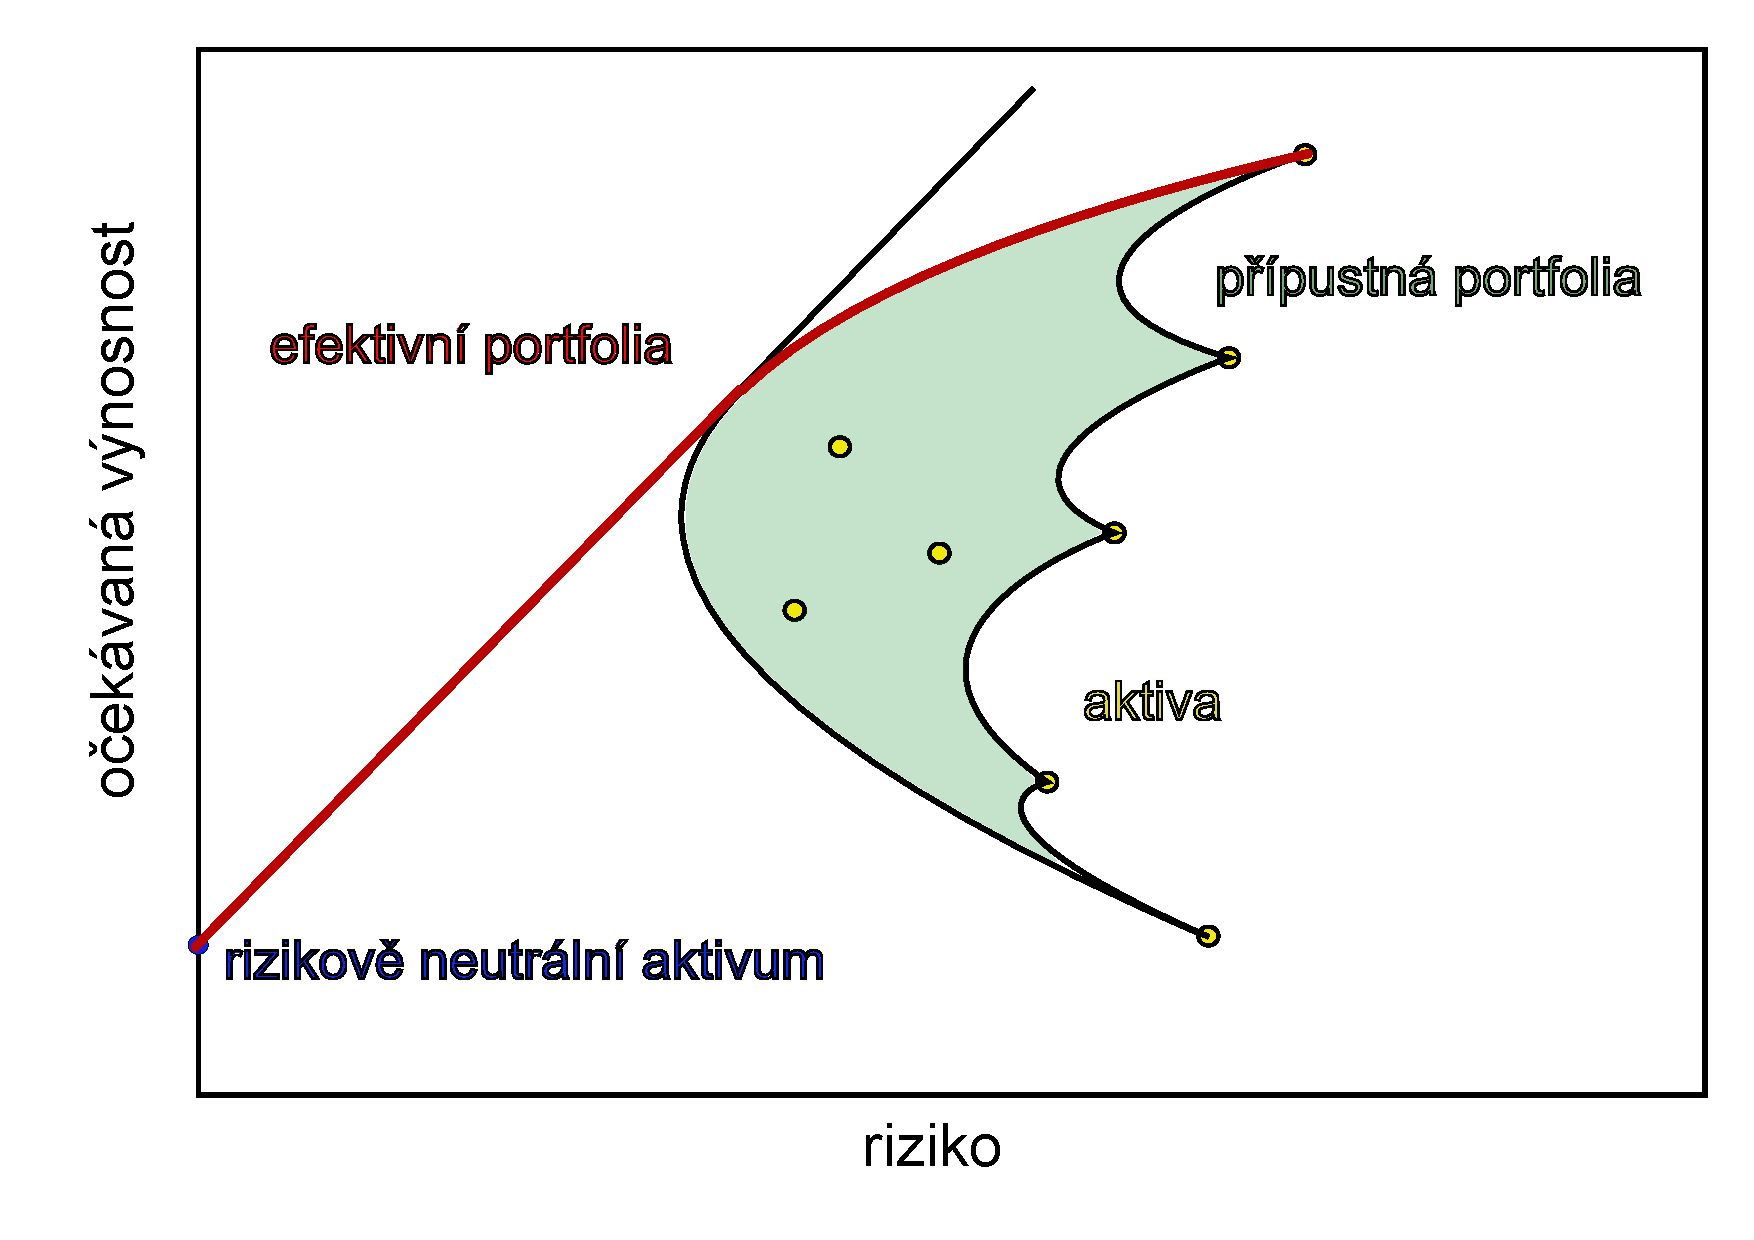
\includegraphics[width=7cm]{IMG/graf_5b.pdf}
  %\caption{}
 \end{figure}
\end{frame}

\begin{frame}
  \frametitle{Tobinův model}
  \begin{itemize}
   \item tangenciální portfolio 
  \end{itemize} 
  
  \begin{figure}[!htbp]
  \centering 
  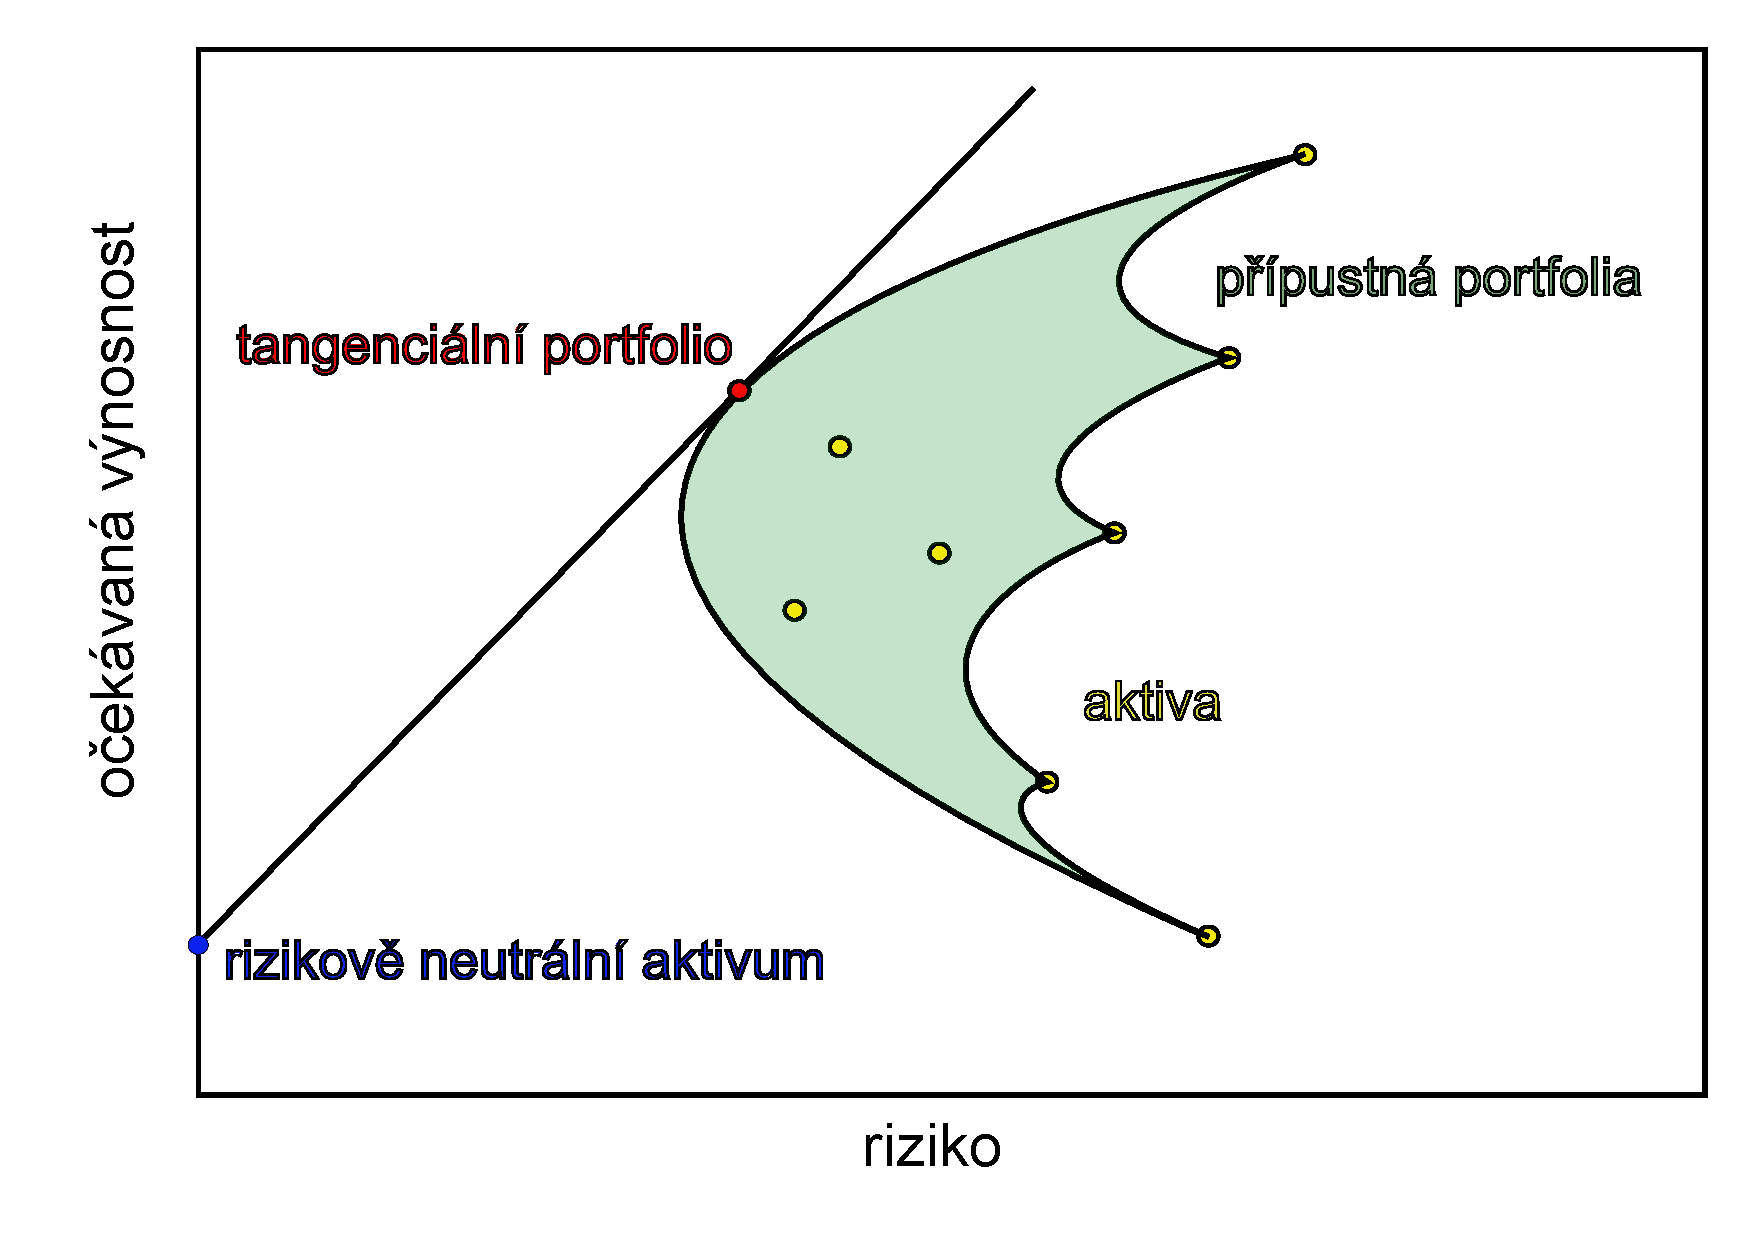
\includegraphics[width=7cm]{IMG/graf_1.pdf}
  %\caption{}
 \end{figure}
\end{frame}

\begin{frame}
  \frametitle{Tobinův model}
  \begin{itemize}
   \item tangenciální portfolio $\to$ separační věta
  \end{itemize} 
  
  \begin{figure}[!htbp]
  \centering 
  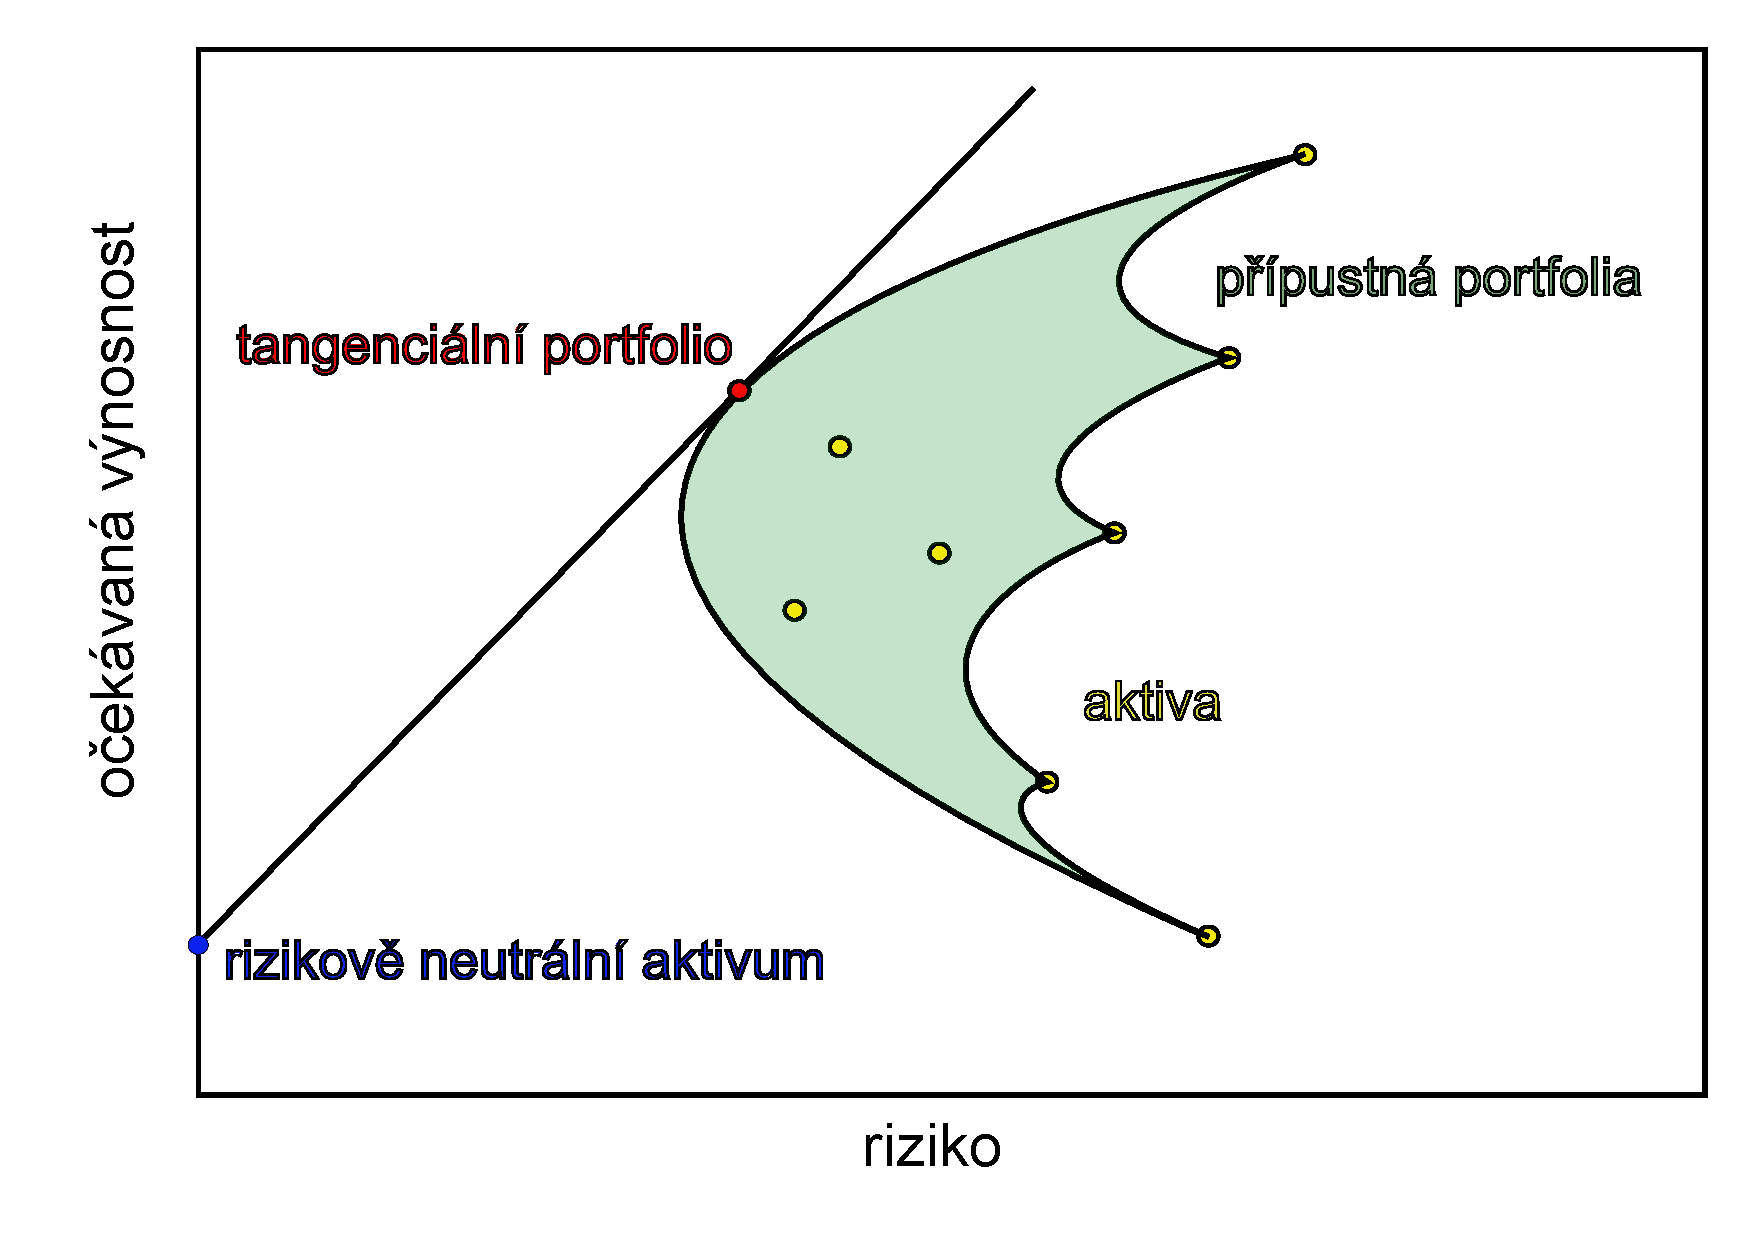
\includegraphics[width=7cm]{IMG/graf_1.pdf}
  %\caption{}
 \end{figure}
\end{frame}

\subsection{CAPM - model oceňování kapitálových aktiv}

\begin{frame}
  \frametitle{CAPM}
  \begin{itemize}
   \item zkoumá chování trhu
   \item vychází z Tobinova modelu
  \end{itemize}  
\vfill
 \textcolor{OliveGreen}{Předpoklady modelu:}
 \begin{itemize}
   \item investoři při sestavování portfolia využívají Markowitzův přístup
   \item investoři mají homogenní očekávání
  \end{itemize}  
\end{frame}

\begin{frame}
  \frametitle{CAPM}
  \begin{itemize}
   \item tržní portfolio 
  \end{itemize} 
  
  \begin{figure}[!htbp]
  \centering 
  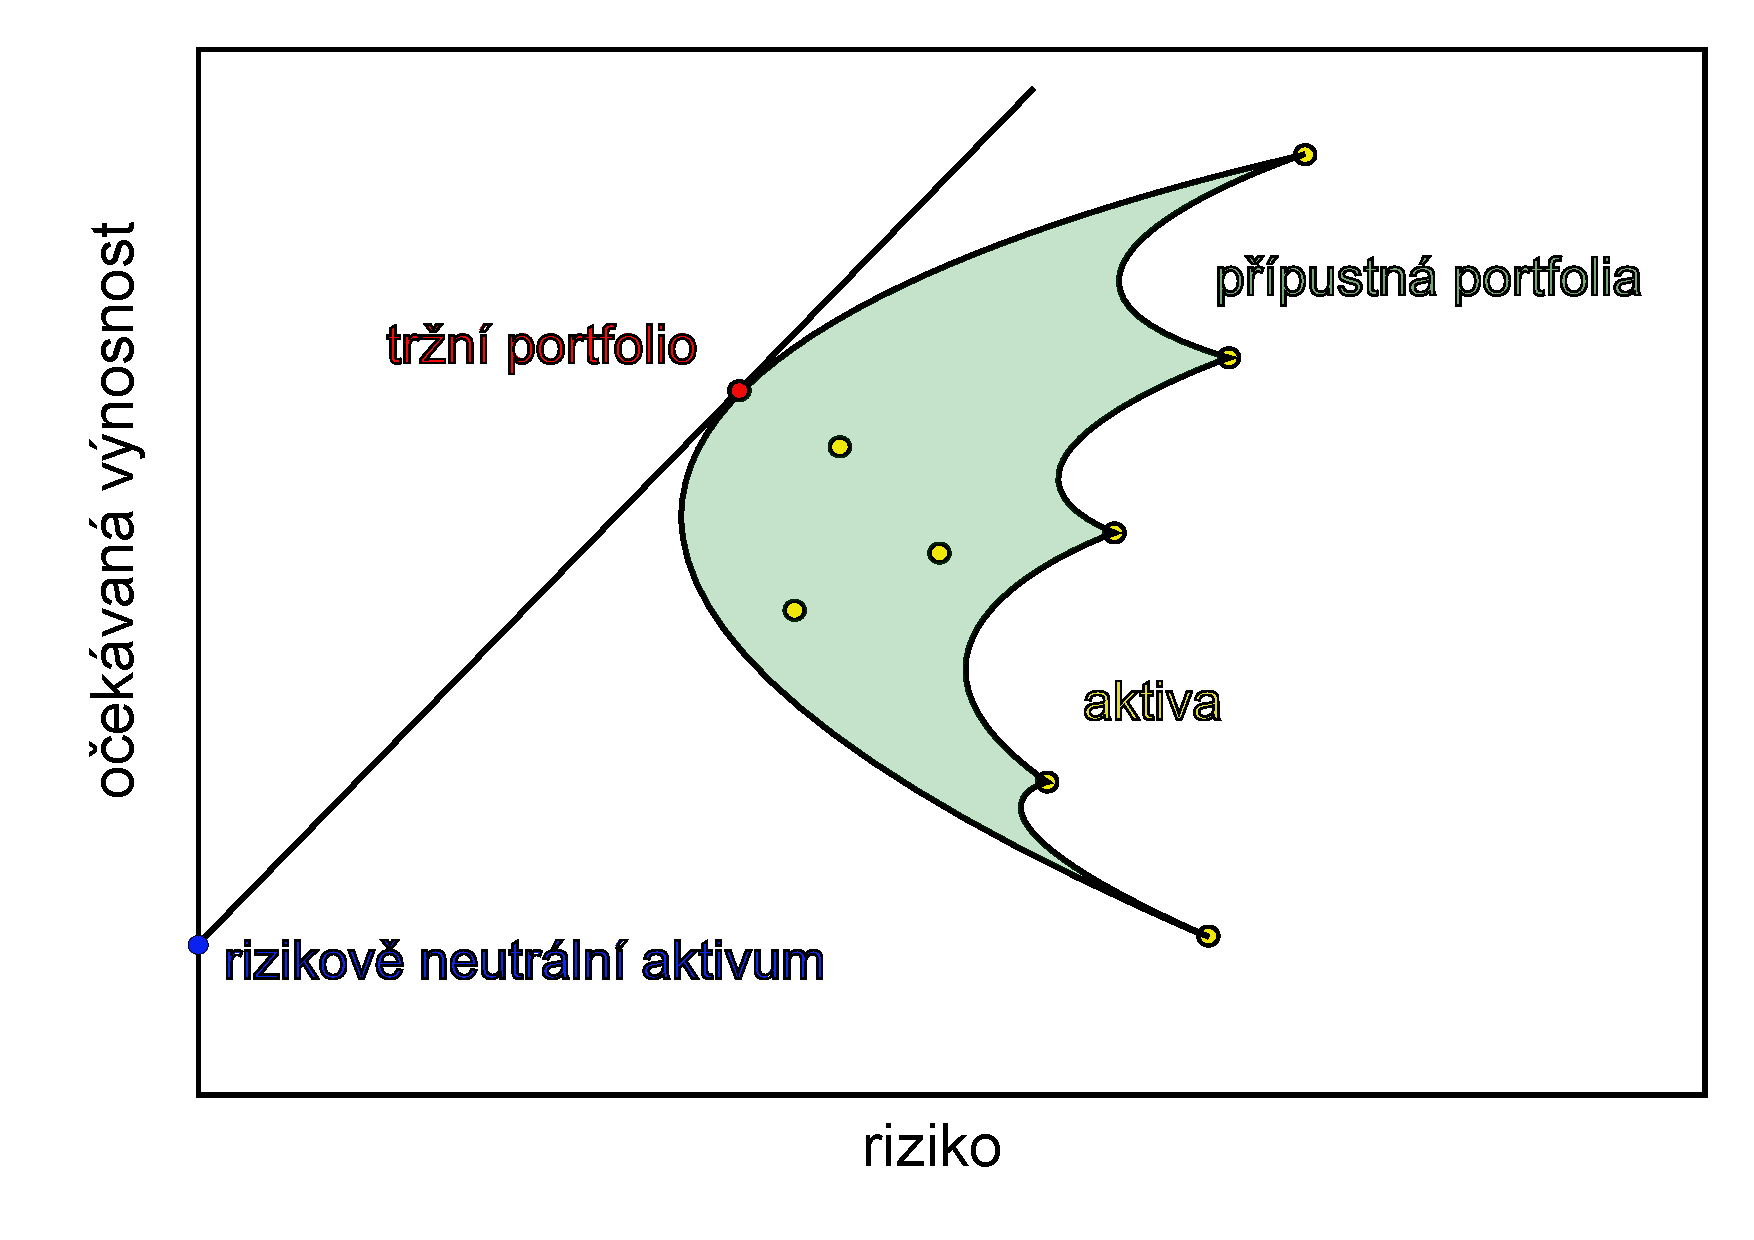
\includegraphics[width=7cm]{IMG/graf_CAPM.pdf}
  %\caption{}
 \end{figure}
\end{frame}

\begin{frame}
  \frametitle{Důsledky CAPM}
Důsledkem CAPM je \textcolor{OliveGreen}{tržní rovnováha} a \textcolor{OliveGreen}{separační věta}. 

 \begin{veta}[Separační věta]
  Všichni investoři drží portfolia se stejnými relativními podíly rizikových aktiv bez ohledu na svou rizikovou averzi a své portfolio doplňují bezrizikovým aktivem dle svých rizikových preferencí.
 \end{veta}

  \begin{definice}[Tržní rovnováha]
  Pojem \textit{tržní rovnováha} označuje takovou situaci, při které je nabídka vyrovnána s poptávkou.
  \end{definice}
\end{frame}

\begin{comment}
\begin{frame}
  \frametitle{Dynamická tržní rovnováha}
  \begin{definice}[Dynamická rovnováha]
  Kapitálový trh je v \textit{dynamické rovnováze} právě tehdy, když
  v~každém čase $t$, pro každé aktivum $j$ a každého investora $i$ existuje vektor cen aktiv $\boldsymbol{P}(t)$ takový, že
  $$\sum_{i\in I} w_{j}(i,t)=N_j(t)P_j(t)=V_j(t),$$
 kde $V_j(t)$ je tržní hodnota aktiva $j$ v čase $t$ a $ w_{j}(i,t)$ je optimální množství bohatství investované investorem $i$ do aktiva $j$ v~čase~$t$.\\
  Ceny $\boldsymbol{P}(t)$ se nazývají  \textit{tržní ceny}.
  \end{definice}
\end{frame}
\end{comment}


\section{Dynamická teorie portfolia}

\begin{frame}
  \frametitle{Klasická teorie portfolia \textcolor{LimeGreen}{x} Dynamická teorie portfolia}
 \centering 
 \begin{tabular}{|r||c|c|}  \hline
  & \textcolor{OliveGreen}{Klasická teorie} &\textcolor{OliveGreen}{Dynamická teorie} \\
  & \textcolor{OliveGreen}{portfolia} &\textcolor{OliveGreen}{portfolia} \\
  \hline
   čas & diskrétní & spojitý  \\   \hline
  výhody & intuitivní & realistický  \\   \hline
  nevýhody & nezohledňuje  & složitý  \\
  & změny &   \\ \hline
  \end{tabular}
\end{frame}

%\subsection{Preliminaries}
\subsection{Mertonův model}
\begin{frame}
  \frametitle{Mertonův model}
  \begin{itemize}
   \item předpokládá rovnováhu na trhu (CAPM)
   \item Model pro proces ceny aktiva $P(t)$ je dán
       $$\mathrm{d}P(t)=P(t)\mu\mathrm{d}t+P(t)\sigma\mathrm{d}W(t),$$
      kde $P(t)$ je cena podkladového aktiva v čase $t$ a $W(t)$ je Wienerův proces.
   \item separační věta -- bezrizikové aktivum $\And$ tržní portfolio
  \end{itemize}    %\vspace{1cm}
 \end{frame}
  
 \begin{frame}
  \frametitle{Bezrizikové aktivum $\And$ Tržní portfolio}
   \begin{itemize}
   \item Cena bezrizikového aktiva se řídí následujícím modelem
    $$\mathrm{d}B(t)=B(t)r_f(t)\mathrm{d}t,$$
    kde $B(t)$ je cena bezrizikového aktiva v čase $t$, $r_f(t)$ je míra výnosnosti bezrizikového aktiva.
   
   \item Cena tržního portfolia $P(t)$ se řídí modelem
    $$\mathrm{d}P(t)=P(t)\mu_p\mathrm{d}t+P(t)\sigma_p\mathrm{d}W(t),$$
    kde $W(t)$ je Wienerův proces a $\mu_p$, $\sigma_p$ jsou konstanty. 
  \end{itemize} 
\end{frame}

\begin{frame}
  \frametitle{Optimální portfolio}
Investorovo bohatství $w(t)$ je proces popsaný modelem
$$\frac{\mathrm{d}w(t)}{w(t)}=X_p(t)\frac{\mathrm{d}P(t)}{P(t)}+\big(1-X_p(t)\big)r_f\mathrm{d}t,$$
kde $X_p(t)$ označuje váhu pro tržní portfolio a $X_f=(1-X_p(t))$ označuje váhu pro bezrizikové aktivum. 

\vspace{1cm}
Merton odvodil explicitní řešení pro případ, kdy charakteristiky (očekávaná hodnota a rozptyl) výnosností aktiv jsou konstanty.
\end{frame}

\subsection{Ohlson-Rosenbergův Paradox}
\begin{frame}
  \frametitle{Ohlson-Rosenbergův Paradox}
   \begin{itemize}
   \item Rosenberg and Ohlson (1976)
   \item objevili nekonzistenci Mertonova modelu
   \item rozpor mezi předpoklady: \\
    $\mu_p$, $\sigma_p$ jsou \textcolor{OliveGreen}{konstanty} $\And$ \textcolor{OliveGreen}{tržní rovnováhou}
   \end{itemize} 
\end{frame}

\begin{frame}
  \frametitle{Předpoklady}
  \begin{definice}[Dynamická rovnováha]
  Kapitálový trh je v \textit{dynamické rovnováze} právě tehdy, když
  v~každém čase $t$, pro každé aktivum $j$ a každého investora $i$ existuje vektor cen aktiv $\boldsymbol{P}(t)$ takový, že
  $$\sum_{i\in I} w_{j}(i,t)=N_j(t)P_j(t)=V_j(t),$$
 kde $V_j(t)$ je tržní hodnota aktiva $j$ v čase $t$ a $ w_{j}(i,t)$ je optimální množství bohatství investované investorem $i$ do aktiva $j$ v~čase~$t$.\\
  Ceny $\boldsymbol{P}(t)$ se nazývají  \textit{tržní ceny}.
  \end{definice}
\end{frame}

\begin{frame}
  \frametitle{Předpoklady}
  \begin{definice}[Vlastnost separace]\label{vlastnost_separace}
Vektorová funkce pro optimální alokaci investorových prostředků do všech aktiv na trhu $\boldsymbol{w}(i,t)$ respektuje \textit{vlastnost separace} právě tehdy, když existuje vektor $\boldsymbol{X}=(X_1,\dots,X_n)^\mathrm{T}$ takový, že $\sum_{j=1}^nX_j=1$, a existují skalární parametry $\lambda(i,t)$ takové, že
$$\boldsymbol{w}(i,t)=\lambda(i,t)\boldsymbol{X},$$
pro všechny $i\in I$ a všechny $t\in T$.
\end{definice}
\end{frame}

\begin{frame}
  \frametitle{Rozpor mezi předpoklady}
\begin{veta} \label{T1}
Nechť $\boldsymbol{P}(t)$ pro všechny $t\in T$  jsou rovnovážné ceny.
Dále předpokládejme, že na trhu platí vlastnost separace (definice \ref{vlastnost_separace}).
Pak
\begin{equation}\label{T1_eq}
\mathsf{Pr}\left(\frac{N_j(s)P_j(s)}{N_j(t)P_j(t)}=\frac{N_k(s)P_k(s)}{N_k(t)P_k(t)}\right)=1
\end{equation}
pro všechny časy $s,t\in T$  a pro každé aktivum $j$ a $k$.
\end{veta}

\begin{proof}
Jednoduchý důkaz nalezneme v článku \cite{ohlson}.
\end{proof}
\end{frame}

\begin{frame}
  %\frametitle{}
  \begin{dusledek}
 Budeme-li předpokládat $N_j(t)=N_j$ pro každé aktivum $i$ a všechna $t\in T$,
z předchozí věty plyne
  \begin{align*}
  \mathsf{Pr}\left(r_j(t,t+\Delta t)=r_k(t,t+\Delta t)\right)=1,
  \end{align*}
pro všechna $t\in T$ a pro všechna aktiva $j$ a $k$.
  \end{dusledek}
  
  \vspace{1cm}
Proto jsou aktiva $j$ a $k$ vzájemně dokonale zastupitelné. $\Rightarrow$  \textcolor{OliveGreen}{degenerace trhu}

\end{frame}

\subsection{Stochastická teorie portfolia}

\begin{frame}
  \frametitle{Stochastická teorie portfolia}
   \begin{itemize}
   \item Robert Fernholz (2002)   
   \end{itemize}                  \vspace{0.5cm}
 \textcolor{OliveGreen}{Předpoklady modelu:}
  \begin{itemize}
   \item parametry procesu ceny aktiva jsou také stochastické procesy
   \item nepředpokládá tržní rovnováhu
   \item nepředpokládá neexistenci arbitráže 
 \end{itemize}
\end{frame}

\begin{frame}
  \frametitle{Logaritmický model cen aktiv}
Fernholz používá logaritmický model
$$\mathrm{d}\log P_j(t)=\gamma_j(t)\mathrm{d}t+\sum_{k=1}^{n}\xi_{jk}(t)\mathrm{d}W_k(t),$$
kde $P_j(t)$ je cena aktiva $j$ v čase $t$, $\gamma_j(t)$ a $\xi_{jk}(t)$ jsou stochastické procesy a $\boldsymbol{W}(t)=(W_1(t),\dots,W_n(t))^\mathrm{T}$ je $n$-rozměrný Wienerův proces. 

\begin{itemize}
   \item  $\gamma_j(t)$ se nazývá \textit{tempo růstu}
   \item  $\xi_{jk}(t)$ se nazývá proces \textit{volatility} 
 \end{itemize}     
\end{frame}

\begin{frame}
  \frametitle{Tempo růstu a volatilita}
  \begin{itemize}
  \item Tempo růstu a míra výnosnosti jsou spolu ve vztahu
        $$\mu_j(t)=\gamma_j(t)+\frac12\sum_{k=1}^{n}{\xi_{jk}}^2(t).$$
  \item Volatilita $\boldsymbol{\xi}$ je maticová odmocnina kovarianční matice $\boldsymbol{\Sigma}$, 
        $$\boldsymbol{\Sigma}=\boldsymbol{\xi}\boldsymbol{\xi}^\mathrm{T}.$$
 \end{itemize}     
\end{frame}

\subsection{Rovnovážný model s výnosností závislou na ceně}

\begin{frame}
  \frametitle{Rovnovážný model s očekávanou výnosností závislou na ceně aktiva}
 \textcolor{OliveGreen}{Předpoklady modelu:}
  \begin{itemize}
   \item očekávaná výnosnost není konstantní (je funkcí ceny)
   \item tržní rovnováha
  \end{itemize}
\end{frame}

\begin{frame}
  \frametitle{Ceny aktiv}
  Předpokládáme, že ceny aktiv splňují stochastickou diferenciální rovnici (SDE)
  \begin{equation} \label{SDE}
 \mathrm{d}P_j(t)=P_j(t)\mu_j(t)\,\mathrm{d}t+P_j(t)\sum_{k=1}^{n}\xi_{jk}(t)\,\mathrm{d}W_k(t),
  \end{equation}
  kde $\boldsymbol{W}(t)=(W_1(t),\dots,W_n(t))^\mathrm{T}$ je $n$-rozměrný Wienerův proces, $\mu_j(t)$ je očekávaná výnosnost aktiva $j$
  a $\xi_{jk}(t)$ jsou volatility aktiv. 
\end{frame}

\begin{frame}
  \frametitle{Váhy tržního portfolia}
  \begin{itemize}
   \item
   Pro vektor vah tržního portfolia uvažujeme následující vztah
    \begin{equation} \label{vahy}
     \boldsymbol{X}=\frac{\boldsymbol{\Sigma}^{-1}\boldsymbol{\mu}}{\boldsymbol{1}^\mathrm{T}\boldsymbol{\Sigma}^{-1}\boldsymbol{\mu}},
    \end{equation}
    kde $\boldsymbol{1}$ je vektor jedniček, $\boldsymbol{\mu}=(\mu_1,\dots,\mu_n)^\mathrm{T}$ je vektor očekávaných výnosností aktiv
    a $\boldsymbol{\Sigma}$ je kovarianční matice výnosností aktiv.
   
   \item váhy tržního portfolia jsou rovny relativní tržní hodnotě
    \begin{equation} \label{market_value}
    \boldsymbol{X}=\frac{\boldsymbol{V}}{\boldsymbol{1}^\mathrm{T}\boldsymbol{V}}
    \end{equation}
  \end{itemize}
\end{frame}

\begin{frame}
  \frametitle{Stochastický proces pro očekávané výnosnosti}
  Rozdělme proces očekávané výnosnosti aktiv na dvě složky:
  \begin{equation} \label{vynos}
\boldsymbol{\mu}(t) =\tilde{\boldsymbol{\mu}}(t)\cdot r(t)
\end{equation}
    \begin{itemize}
   \item  relativní vztahy mezi jednotlivými očekávanými výnosnostmi aktiv v portfoliu ($\tilde{\boldsymbol{\mu}}(t)=\boldsymbol{X}(t)$)
   \item výnosnost celého trhu dynamicky se měnící v čase
   \item multiplikativní vztah
     \end{itemize}
\end{frame}

\begin{frame}
  \frametitle{Vašíčkův model pro míru výnosnosti trhu $r(t)$}
  Výnosnost celého trhu
      \begin{itemize}
   \item nevykazuje exponenciální růst, pohybuje se přibližně v nějakém intervalu
   \item má tendence navracet se k průměrné hodnotě
     \end{itemize}
     \vspace{0.5cm}
     Vašíčkův model pro míru výnosnosti trhu $r(t)$
     \begin{equation} 
\mathrm{d}r(t)=\kappa(\theta-r(t))\,\mathrm{d}t+\sigma\,\mathrm{d}W(t),
\end{equation}
kde $\kappa$, $\theta$ a $\sigma$ jsou konstanty.
\end{frame}

\begin{frame}
  \frametitle{Zjednodušující předpoklady pro SDE cen aktiv}
 \textcolor{OliveGreen}{Předpoklady modelu:}
  \begin{itemize}
  % \item matice $\boldsymbol{\Sigma}$ je diagonální
   \item volatility aktiv $\xi_{jk}$ jsou konstantní v čase
   \item počty aktiv $N_j$ jsou konstantní v čase
  \end{itemize}    \vspace{1cm}
  Z těchto předpokladů a z SDE \eqref{SDE} dostáváme
\begin{equation} 
 \mathrm{d}P_j(t)=P_j(t)\left(\frac{P_j(t)N_j}{\sum_{i=1}^n P_i(t)N_i}\, r(t)\right)\,\mathrm{d}t+P_j(t)\sum_{k=1}^{n}\xi_{jk}\,\mathrm{d}W_k(t).
\end{equation}  
Soustava je nelineární a neexistuje její analytické řešení.
\end{frame}

\begin{comment}
\begin{frame}
  \frametitle{Zjednodušující předpoklady pro SDE cen aktiv}
 \textcolor{OliveGreen}{Předpoklady modelu:}
  \begin{itemize}
   \item matice $\boldsymbol{\Sigma}$ je diagonální
   \item rizika aktiv $\sigma_j$ jsou konstantní
   \item počety aktiv $N_j$ jsou konstantní
  \end{itemize}    \vspace{1cm}
  Z těchto předpokladů a z SDE \eqref{SDE} dostáváme
  $$ \mathrm{d}P_j(t)=P_j^2(t){\sigma_{j}}^2N_j\mathrm{d}t+P_j(t)\sigma_{j}\mathrm{d}W_j(t).$$
\end{frame}

\begin{frame}
  \frametitle{Očekávaná cena aktiva}
Hledáme vztah pro očekávanou cenu aktiva.
\begin{equation*}
\mathsf{E}\big(\mathrm{d}P_j(t)\big)=\mathsf{E}\big(P_j^2(t){\sigma_{j}}^2N_j\mathrm{d}t\big)
\end{equation*}  
 \pause 
Úpravami získáme obyčejnou diferenciální rovnici (ODE)
\begin{align*}
\mathrm{d}\mathsf{E}\big(P_j(t)\big)&={\sigma_{j}}^2N_j\mathsf{E}\big(P_j^2(t)\big)\mathrm{d}t\\
&={\sigma_{j}}^2N_j\big[\mathsf{D}\big(P_j(t)\big)+\mathsf{E}^2\big(P_j(t)\big)\big]\mathrm{d}t\\
&={\sigma_{j}}^2N_j\big[{\sigma_{j}}^2+\mathsf{E}^2\big(P_j(t)\big)\big]\mathrm{d}t \\\\\\
\end{align*}  
\end{frame}

\begin{frame}
  \frametitle{Očekávaná cena aktiva}
Hledáme vztah pro očekávanou cenu aktiva.
\begin{equation*}
\mathsf{E}\big(\mathrm{d}P_j(t)\big)=\mathsf{E}\big(P_j^2(t){\sigma_{j}}^2N_j\mathrm{d}t\big)
\end{equation*}  
 
Úpravami získáme obyčejnou diferenciální rovnici (ODE) 
\begin{align*}
\underline{\mathrm{d}\mathsf{E}\big(P_j(t)\big)}&={\sigma_{j}}^2N_j\mathsf{E}\big(P_j^2(t)\big)\mathrm{d}t\\
&={\sigma_{j}}^2N_j\big[\mathsf{D}\big(P_j(t)\big)+\mathsf{E}^2\big(P_j(t)\big)\big]\mathrm{d}t\\
&\underline{={\sigma_{j}}^2N_j\big[{\sigma_{j}}^2+\mathsf{E}^2\big(P_j(t)\big)\big]\mathrm{d}t}
\end{align*}  
\pause
Řešení ODE je
\begin{equation*} 
\boxed{\mathsf{E}\big(P_j(t)\big)=\sigma_j\mathrm{tan}\big({\sigma_j}^3N_jt\big)}.
\end{equation*}
\end{frame}

%\begin{frame}
%  \frametitle{Bubbles in the Market}
%\begin{equation*} 
%\mathsf{E}\big(P_j(t)\big)=\sigma_j\mathrm{tan}\big({\sigma_j}^3N_jt\big)
%\end{equation*}
% \begin{itemize}
%   \item for ${\big(\sigma_j}^3N_jt\big)\to\frac\pi2$ is $\mathsf{E}\big(P_j(t)\big)\to\infty$ 
%   \item the behavior of price bubbles in the market
% \end{itemize}     
%    
%  \begin{figure}[!htbp]
%  \centering 
%  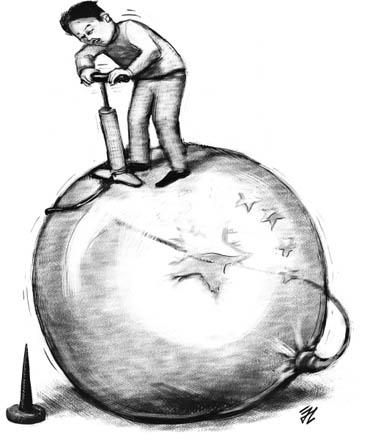
\includegraphics[width=3cm]{IMG/stock-bubble.jpg}
  %\caption{}
% \end{figure}
%\end{frame}

\begin{frame}
  \frametitle{Předpoklady pro SDE cen aktiv}
 \textcolor{OliveGreen}{Předpoklady modelu:}
  \begin{itemize}
   \item matice $\boldsymbol{\Sigma}$ \sout{je diagonální}
   \item rizika aktiv $\sigma_j$ jsou konstantní
   \item počety aktiv $N_j$ jsou konstantní
  \end{itemize}    \vspace{1cm}
  Z těchto předpokladů a z SDE \eqref{SDE} dostáváme
\begin{equation*} 
 \mathrm{d}P_j(t)=P_j(t)\sum_{k=1}^{n}P_k(t)N_k(t)\sigma_{jk}\mathrm{d}t+P_j(t)\sum_{k=1}^{n}\xi_{jk}(t)\mathrm{d}W_k(t).
\end{equation*}
\end{frame}


\begin{frame}
  \frametitle{Očekávaná cena aktiva}
Hledáme vztah pro očekávanou cenu aktiva.
\begin{equation*} 
\mathsf{E}\big( \mathrm{d}P_j(t)\big)=\mathsf{E}\left(P_j(t)\sum_{k=1}^{n}P_k(t)N_k(t)\sigma_{jk}\mathrm{d}t\right)
\end{equation*}

Úpravami získáme systém diferenciálních rovnic
\begin{align*}
\mathrm{d}\mathsf{E}\big(P_j(t)\big)&=N_j\left[\sum_{k=1}^{n}{\sigma_{jk}}^2+\mathsf{E}\big(P_j(t)\big)\sum_{k=1}^{n}\sigma_{jk}\mathsf{E}\big(P_k(t)\big)\right]\mathrm{d}t
\end{align*}  
\end{frame}
\end{comment}

\begin{frame}
  \frametitle{Data}
    \begin{itemize}
    \item ČEZ -  {\scriptsize(největší výrobce elektřiny v Česku)}
    \item O2 -  {\scriptsize(český telefonní operátor ve vlastnictví PPF)}
    \item KB -  {\scriptsize(český bankovní ústav)}
    \item PM - Philip Morris ČR a.s. {\scriptsize(přední výrobce a prodejce cigaret v Česku)}
    \item Pegas - Pegas Nonwovens s.r.o. {\scriptsize(přední světový výrobce netkaných textilií se sídlem v ČR)}
    \item ČT -  Česká televize {\scriptsize(veřejnoprávní televize)}
    \item NWR -  New World Resources {\scriptsize(přední producent černého uhlí ve střední Evropě)}
    \end{itemize}
\end{frame}

\begin{frame}
  \frametitle{Ceny aktiv}
 \begin{figure}[!htbp]
  \centering 
	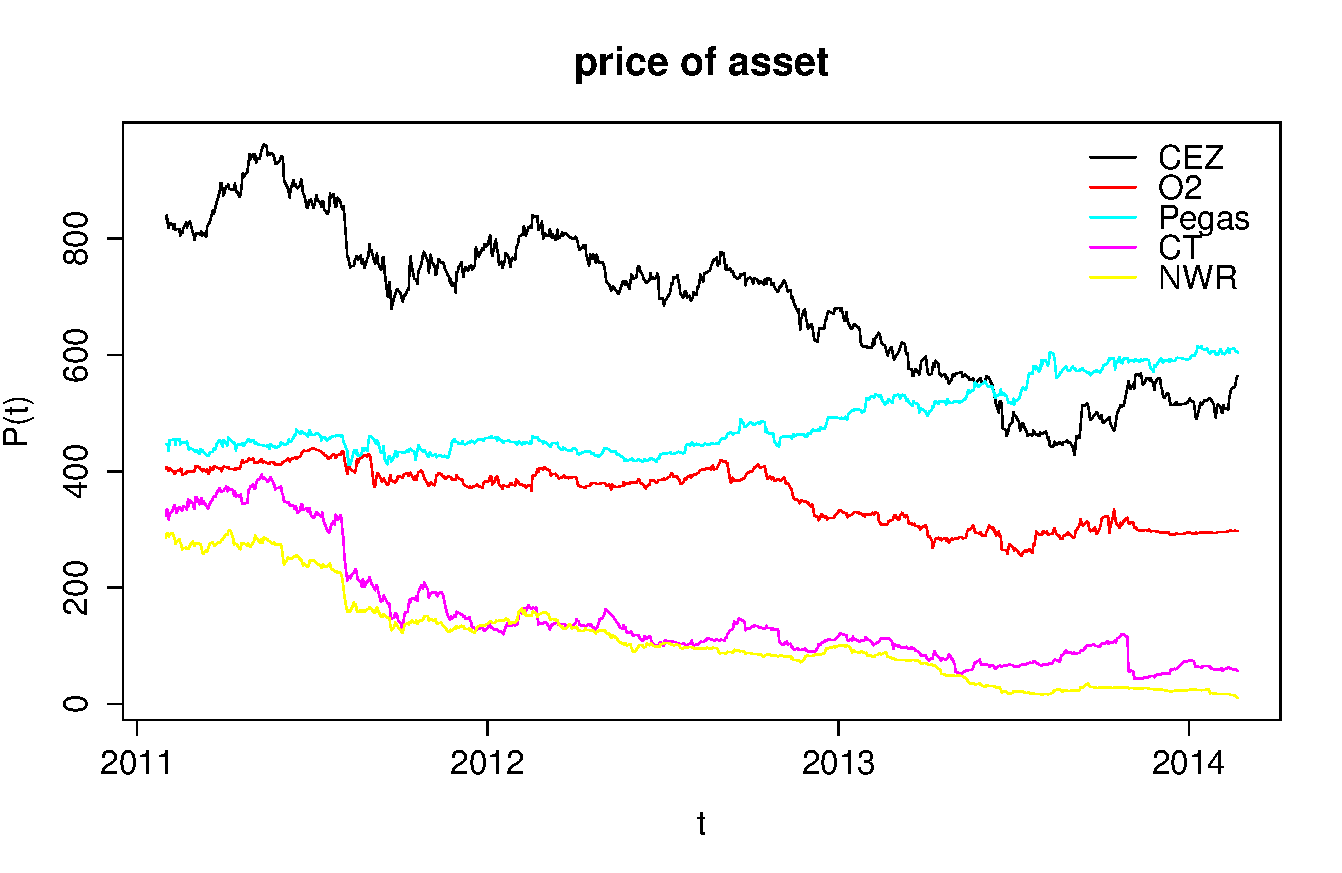
\includegraphics[width=5cm, clip, trim= 0 15 25 50]{IMG/data_price_of_asset_ostatni.pdf}\\[5mm]
	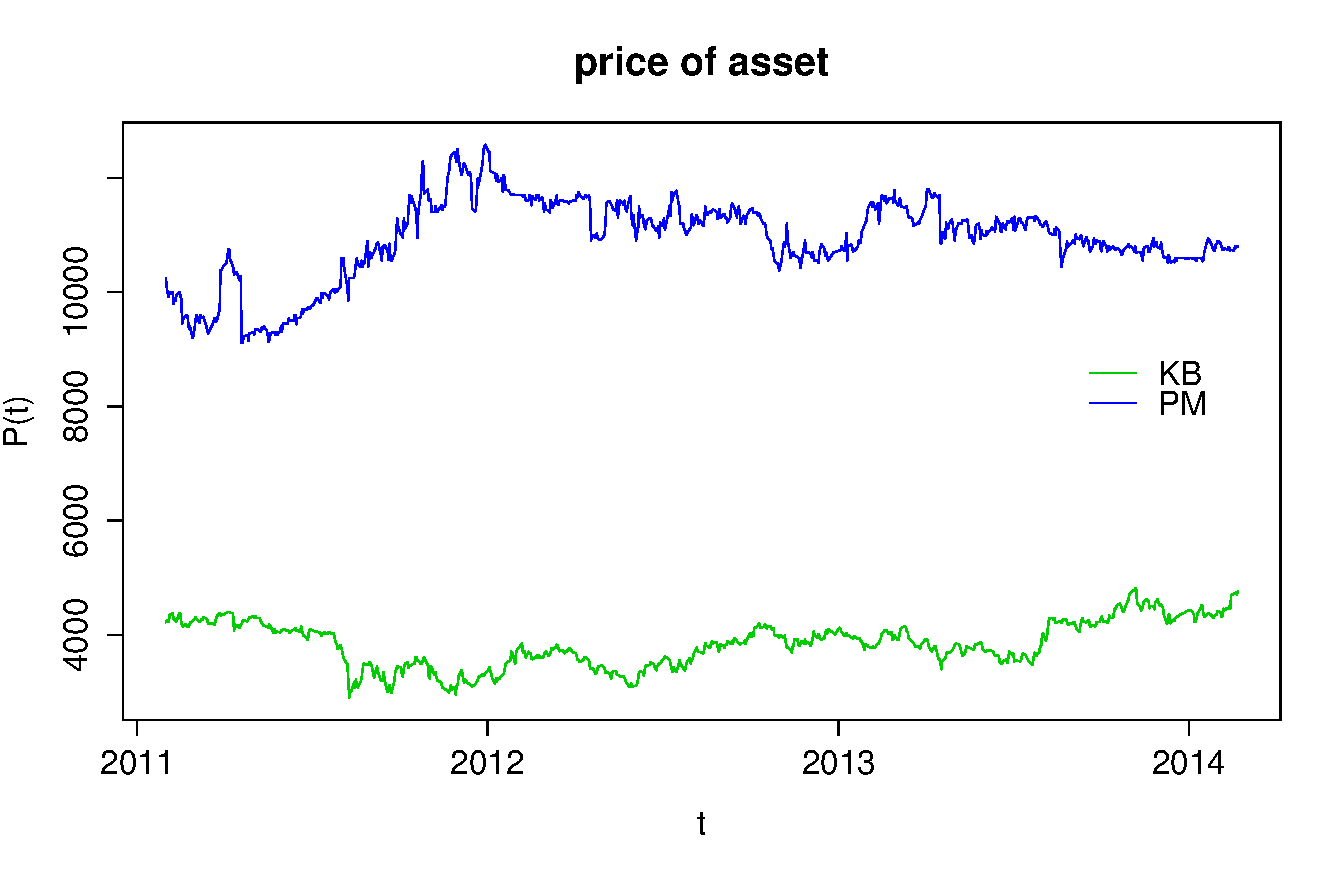
\includegraphics[width=5cm, clip, trim= 0 15 25 50]{IMG/data_price_of_asset_KBPM_v2.pdf}	
  %\caption{Ceny aktiv v portfoliu}  \label{model_price_of_asset}
\end{figure} 
\end{frame}


\begin{frame}
  \frametitle{Eulerova metoda}
  Eulerova metoda řešení soustavy SDR je pro $i$-tou složku rovnice definována rekurzívním vztahem
\begin{equation}
X_{n+1}^i=X_n^i+\alpha^i(t_n,\boldsymbol{X}_n)\Delta_n+\sum_{j=1}^m\beta^{i,j}(t_n,\boldsymbol{X}_n)\Delta W_n^j,
\end{equation}
kde $\Delta_n=\int_{t_n}^{t_{n+1}}\mathrm{d}t=t_{n+1}-t_n$ je délka časového intervalu $(t_n,t_{n+1})$
a $\Delta W_n=\int_{t_n}^{t_{n+1}}\mathrm{d}W(t)=W(t_{n+1})-W(t_n)$ je přírůstek Wienerova procesu $W$ v čase $(t_n,t_{n+1})$.
\end{frame}

\begin{frame}
  \frametitle{Model cen aktiv v portfoliu}
\begin{figure}[!htbp]
  \centering 
	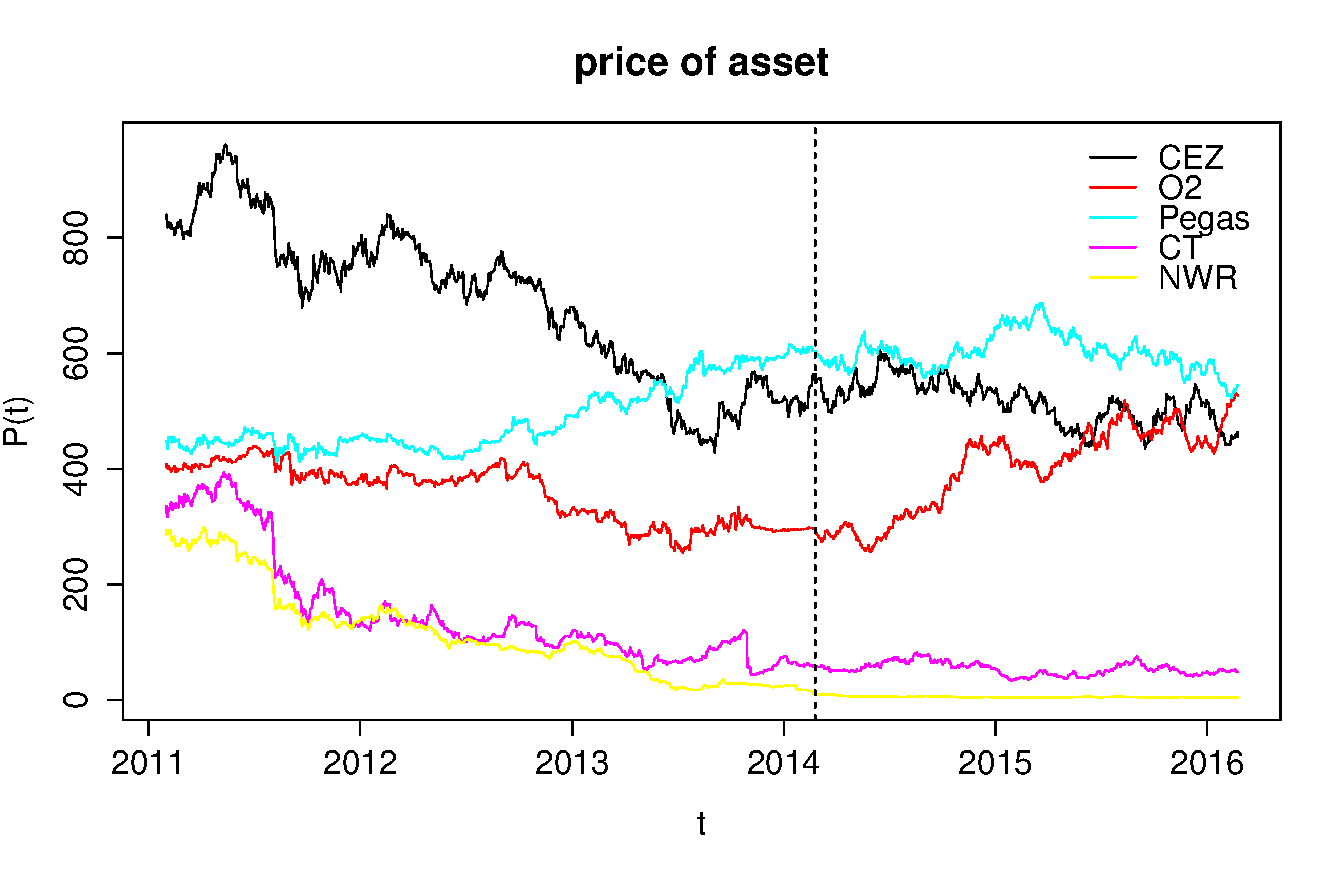
\includegraphics[width=5cm, clip, trim= 0 15 25 50]{IMG/ds_price_of_asset_ostatni.pdf}\\[5mm]
	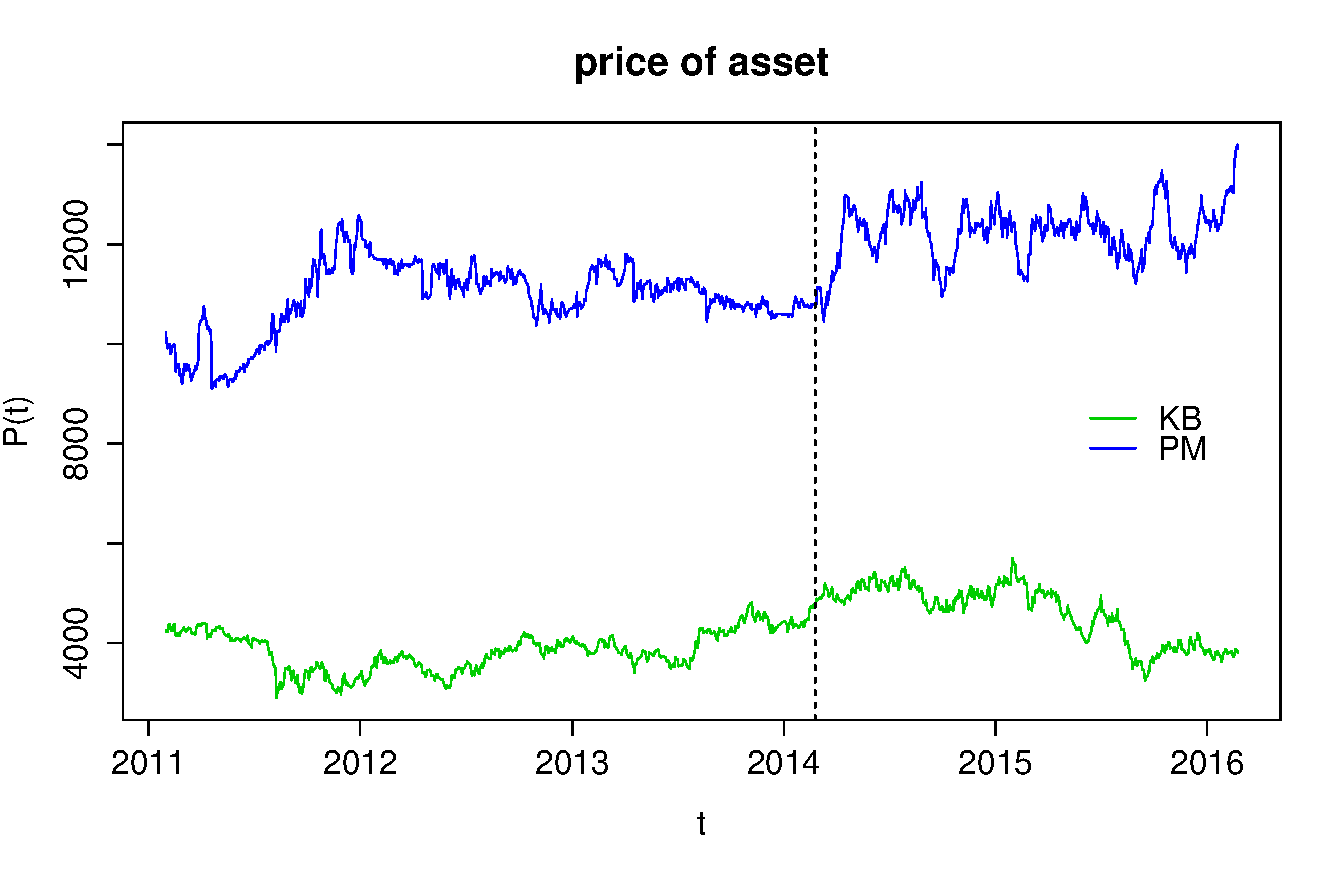
\includegraphics[width=5cm, clip, trim= 0 15 25 50]{IMG/ds_price_of_asset_KBPM_v2.pdf}	
%  \caption{Model cen aktiv v portfoliu}  \label{price_of_asset}
\end{figure}  
\end{frame}

\begin{frame}
  \frametitle{Kam dál?}
\begin{figure}[h]
   \centering
   \begin{minipage}[c]{0.3\textwidth}
     \centering 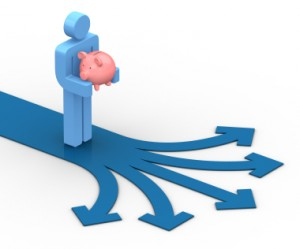
\includegraphics[width=4cm]{IMG/rozcesti.jpg}
   \end{minipage}
\hfill
   \begin{minipage}[c]{0.6\textwidth}
  \begin{itemize}
   \item odhad střední hodnoty a rozptylu ceny aktiva ze simulací
   \item jiné numerické metody  
   %\item simulace  \textcolor{LimeGreen}{x} reálná data
   \item jiný odhad $\boldsymbol{\xi}$%\quad $\boldsymbol{\Sigma}=\boldsymbol{\xi}\boldsymbol{\xi}^\mathrm{T}$
   \item ???
  \end{itemize}
   \end{minipage}	
   \end{figure}
\end{frame}

\begin{comment}
\begin{frame}
  \frametitle{}
\end{frame}
\end{comment}

\section<presentation>*{Literatura}
\subsection{}
\begin{frame}
  \frametitle<presentation>{Literatura}
  \beamertemplatebookbibitems
 \begin{thebibliography}{99}
 \bibitem[Fabozzi et al. (2008)]{fabozzi} FABOZZI, F. J. et al. 2008. \textit{Bayesian Methods in Finance}. Hoboken, New Jersey: John Wiley \& Sons. ISBN 978-0-471-92083-0.

 \bibitem[Fernholz (2002)]{fern} FERNHOLZ, E. R., 2002. \textit{Stochastic Portfolio Theory}. New York: Springer-Verlag. ISBN 0-387-95405-8.

 \beamertemplatearticlebibitems
 %\bibitem[Karatzas and Fernholz (2009)]{kara} KARATZAS, I., FERNHOLZ, R., 2009.  Stochastic Portfolio Theory: an Overview. {\it Handbook of Numerical Analysis.} 15, p.~89--167.

 \bibitem[Merton (1971)]{merton} MERTON, R. C., 1971.  Optimum Consumption and Portfolio Rules in a Continuous-Time Model. {\it Journal of Economic Theory.} 3, p.~373--413.

 \bibitem[Rosenberg and Ohlson (1976)]{ohlson} ROSENBERG, B., OHLSON, J. A., 1976.  The Stationary Distribution of Returns and Portfolio Separation in Capital Markets: A Fundamental Contradiction. {\it Journal of Financial and Quantitative Analysis.} 11, p.~393--402.

 %\bibitem[Tobin (1958)]{tobin} TOBIN, J., 1958.  Liquidity Preference as Behavior Towards Risk. {\it Review of Economic Studies.} 25, p.~65--86.

 \end{thebibliography}
\end{frame}


\begin{frame}
 \vfill
 \begin{center}
  \textcolor{OliveGreen}{\Large{Děkuji za pozornost.}}
 \end{center}
 \begin{figure}[!htbp] 
 \centering
 
\includegraphics[width=3.5cm]{IMG/silak.jpg}
\end{figure} 
 \vfill
\end{frame}

\end{document}